\documentclass[a4paper, 12pt]{book}
%\usepackage[T1]{fontenc}


\usepackage[a4paper, left=2.5cm, right=2.5cm, top=3cm, bottom=3cm]{geometry}
\usepackage{times}
%\usepackage[latin1]{inputenc}
\usepackage[spanish]{babel} %comentar linea si tu memoria es en ingles.
\selectlanguage{spanish}
\usepackage[utf8]{inputenc}
\usepackage{url}
%\usepackage[dvipdfm]{graphicx}
\usepackage{graphicx}
\usepackage{float} %% H para posicionar figuras
\usepackage[nottoc, notlot, notlof, notindex]{tocbibind} %% Opciones de indice.
\usepackage{latexsym} %% Logo de LaTeX
\usepackage{multirow} %% Para las tablas
\usepackage{pdfpages}
\usepackage{listings} %% para el codigo

\title{Memoria del Proyecto}
\author{Nombre del autor}

\renewcommand{\baselinestretch}{1.5} %%Interlineado

\begin{document}

\renewcommand{\refname}{Bibliografía}  %%Renombrado
\renewcommand{\appendixname}{Apéndice}

%%%%%%%%%%%%%%%%%%%%%%%%%%%%%%%%%%%%%%%%%%%%%%%%%%%%%%%%%%%%%%%%%%
% PORTADA

\begin{titlepage}
\begin{center}
\begin{tabular}[c]{c c}


\includegraphics[scale=0.25]{img/logo_vect.png}&
\begin{tabular}[b]{l}
\Huge
\textsf{UNIVERSIDAD}  \\
\Huge
\textsf{REY JUAN CARLOS} \\
\end{tabular}
\\
\end{tabular}

\vspace{3cm}

\large
GRADO EN INGENIER\'IA DE SISTEMAS AUDIOVISUALES Y MULTIMEDIA

\vspace{0.4CM}

\large
Curso Académico 2019/2020

\vspace{0.8cm}
Trabajo Fin de Grado

\vspace{2.5cm}

\large
IMPLEMENTACI\'ON DE UN PLUGIN DE VISUALIZACI\'ON EN REALIDAD VIRTUAL EN KIBANA
\vspace{4cm}

\large
Autor: Andrea Villaverde Hern\'andez

Tutor: Dr. Jes\'us Mar\'ia Gonzalez Barahona
\end{center}
\end{titlepage}

\newpage
\mbox{}
\thispagestyle{empty} % para que no se enumere la página

%%%%%%%%%%%%%%%%%%%%%%%%%%%%%%%%%%%%%%%%%%%%%%%%%%%%%%%%%%%%%%%%%%
% FIRMAS

\clearpage
\pagenumbering{gobble}
\chapter*{}

\vspace{-4cm}
\begin{center}
\large
\textbf{Trabajo Fin de Grado}

\vspace{1cm}
\large
IMPLEMENTACI\'ON DE UN PLUGIN DE VISUALIZACI\'ON EN REALIDAD VIRTUAL EN KIBANA

\vspace{1cm}
\large
\textbf{Autor :} Andrea Villaverde Hern\'andez \\
\textbf{Tutor :} Dr. Jes\'us Mar\'a Gonzalez Barahona

\end{center}

\vspace{1cm}
La defensa del presente Proyecto Fin de Grado se realiz\'o el d\'ia \qquad$\;\,$ de \qquad\qquad\qquad\qquad \newline de 2020, siendo calificada por el siguiente tribunal:

\vspace{0.5cm}
\textbf{Presidente:}

\vspace{1.2cm}
\textbf{Secretario:}

\vspace{1.2cm}
\textbf{Vocal:}

\vspace{1.2cm}
y habiendo obtenido la siguiente calificaci\'on:

\vspace{1cm}
\textbf{Calificaci\'on:}


\vspace{1cm}
\begin{flushright}
Fuenlabrada, a \qquad$\;\,$ de \qquad\qquad\qquad\qquad de 2020
\end{flushright}

%%%%%%%%%%%%%%%%%%%%%%%%%%%%%%%%%%%%%%%%%%%%%%%%%%%%%%%%%%%%%%%%%
% DEDICATORIA

\chapter*{}
\pagenumbering{Roman} % para comenzar la numeracion de paginas en números romanos.
\begin{flushright}
\textit{Dedicado a \\ 
todos aqu\'ellos que \\
nunca se rindieron.}
\end{flushright}

%%%%%%%%%%%%%%%%%%%%%%%%%%%%%%%%%%%%%%%%%%%%%%%%%%%%%%%%%%%%%%%%
% AGRADECIMIENTOS

\chapter*{Agradecimientos}
\markboth{AGRADECIMIENTOS}{AGRADECIMIENTOS} %Encabezado

Gracias a...

\textit{<<If you can dream it, you can do it.>> - Walter Elias Disney}

%%%%%%%%%%%%%%%%%%%%%%%%%%%%%%%%%%%%%%%%%%%%%%%%%%%%%%%%%%%%%%%%
% RESUMEN

\chapter*{Resumen}
\markboth{RESUMEN}{RESUMEN} %Encabezado

Este proyecto...

%%%%%%%%%%%%%%%%%%%%%%%%%%%%%%%%%%%%%%%%%%%%%%%%%%%%%%%%%%%%%%%%%
% RESUMEN EN INGLÉS

\chapter*{Summary}
\markboth{SUMMARY}{SUMMARy} %Encabezado

This...

%%%%%%%%%%%%%%%%%%%%%%%%%%%%%%%%%%%%%%%%%%%%%%%%%%%%%%%%%%%%%%%%%
% ÍNDICES %
%%%%%%%%%%%%%%%%%%%%%%%%%%%%%%%%%%%%%%%%%%%%%%%%%%%%%%%%%%%%%%%%%

% Lo índices se generan automáticamente
% Solo hay que comentar/descomentar la instrucción de LaTeX.

%%%% Índice de contenidos
\tableofcontents
%%%% Índice de figuras
\cleardoublepage
\listoffigures % lista de figuras




%%%%%%%%%%%%%%%%%%%%%%%%%%%%%%%%%%%%%%%%%%%%%%%%%%%%%%%%%%%%%%%%%
% INTRODUCCION %
%%%%%%%%%%%%%%%%%%%%%%%%%%%%%%%%%%%%%%%%%%%%%%%%%%%%%%%%%%%%%%%%%

\cleardoublepage
\chapter{Introducci\'on}
\label{sec:intro} %etiqueta para referenciar luego ~\ref{sec:intro}
\pagenumbering{arabic} %para empezar enumeracion con numeros

% hablar sobre los objetivos del proyecto

\section{El problema}
\label{sec:ElProblema}

%%%%%%%%%%%%%%%%%%%%%%%%%%%%%%%%%%%%%%%%%%%%%%%%%%%%%%%%%%%%%%%%%
% CONTEXTO Y TECNOLOGIAS USADAS %
%%%%%%%%%%%%%%%%%%%%%%%%%%%%%%%%%%%%%%%%%%%%%%%%%%%%%%%%%%%%%%%%%

\cleardoublepage
\chapter{Contexto y tecnolog\'ias utilizadas}
\label{sec:tecno} %etiqueta para referenciar luego 

% motivaciones y hablar sobre las herramientas

%%%%%%%%%%%%%%%
%HTML5
%%%%%%%%%%%%%%%

\section{HTML5}
\label{sec:html5}
\subsection{Definici\'on}
\subsection{En este proyecto}

%%%%%%%%%%%%%%%
%JAVASCRIPT
%%%%%%%%%%%%%%%

\section{JavaScript}
\label{sec:js}
\subsection{Definici\'on}
\subsection{En este proyecto}

%%%%%%%%%%%%%%%%
%AFRAME
%%%%%%%%%%%%%%%

\section{A-Frame}
\label{sec:aframe}
\subsection{Definici\'on}
A-frame es un framework web que permite la creaci\'on de experiencias VR (Realidad Virtual). Desarrollado por Mozilla pensado para implementar contenido VR a nuestra web de manera sencilla, sin la necesidad de instalar nada. Se trata de un proyecto de C\'odigo Abierto, por lo que ha sido muy bien recibido en las comunidades VR.

A primera vista, A-frame parece de f\'acil manejo; pues permite la creaci\'on de escenarios 3D utilizando simple etiquetas HTML. Pero no todo esto se queda aqu\'i, pues es un poderoso framework de entity-component que viene dado por su fichero three.js.

A-Frame soporta dispositivos de VR como Vive, Rift, Daydream, Gear VR o Cardboard.
Adem\'as, gracias a dispositivos de tracking y controladores de posici\'on, permite sumergirse en experiencias VR en escenarios a 360\textsuperscript{\underline{o}}.
\subsubsection{Caracter\'isticas}
\begin{itemize}
\item \underline{Crea VR de forma sencilla}: simplemente utilizando las etiquetas <<script>> y <<a-scene>> podr\'as crear un escenario 3D con toda la configuraci\'on para VR, de forma predeterminada, sin la necesidad de instalar nada.
\item \underline{Declaraciones en HTML}: al estar basado en HTML es muy f\'acil de usar ya seas desarrollador web, amante del VR, artista, dise~nador, educador o ni~no.
\item \underline{VR Multiplataforma}: permite usar los diferentes dispositivos con sus respectivos controladores. En caso de no disponer de ninguno, tambi\'en se puede usar en port\'atiles, tablets o tel\'efonos  m\'oviles.
\item \underline{Arquitectura Entity-Component}: A-frame es un poderoso framework donde se provee de una poderosa estructura entity-component. Al tratarse de HTML, los desarrolladores tienen acceso ilimitado a javascript, DOM API, three.js, WebVR y WebGL.
\item \underline{Rendimiento}: A-Frame est\'a optimizado desde cero para WebVR. Como A-Frame usa el DOM, sus elementos no tocan el motor del navegador. Los objetos 3D se actualizan en la memoria con una sola llamada ``requestAnimationFrame".
\item \underline{Tool Agnostic}: como la web se crea en HTML, A-frame es compatible con la mayor\'ia de las bibliotecas y herramientas web tales como React, Preact, Vue.js, d3,js, Ember.js y jQuery.
\item \underline{Inspector Visual}: A-frame proporciona un visor 3D incorporado. En la que permite abrir la escena 3D y modificar algunos de sus elementos.
\item \underline{Registro}: al igual que Unity Assets Store, a-Frame recopila componentes para que los desarrolladores puedan publicar y buscarlos de forma sencilla.
\item \underline{Componentes}: con a-Frame se puede correr geometr\'ias, luces, materiales, animaciones, modelos, sombras, audios, texto, etc (adem\'as de los controladores para los dispositivos). Adem\'as de, gracias a su comunidad, sistemas de part\'iculas, f\'isicas, multijugador, aguas, monta~nas, reconocimiento de voz y un gran etc\'etera.
\end{itemize}
\subsection{THREE.JS}
Es una biblioteca escrita en Javascript que permite la creaci\'on y visualizaci\'on de objetos 3D en entornos web. Es muy convenientes pues permite utilizarse en conjunto con Canvas (HTML5) SVG y WebGL. Por lo que podemos decir que es compatible con cualquier navegador que soporte WebGL.

Adem\'as, permite importar modelos 3D, en formato JSON,  creados en Maya, Blender o Max3D.

\subsection{En este proyecto}
A-Frame supone una parte importante de este proyecto, pues el objetivo de este proyecto es crear un plugin que permita dar una experiencia VR a la hora de representar la visualizaci\'on de los datos mostrados en Kibana. 


%%%%%%%%%%%%%%%%%%%
% ELASTICSEARCH
%%%%%%%%%%%%%%%%%%%

\section{ELK}
\label{sec:elastic}
\subsection{Definici\'on}
Es un conjunto de herramientas de gran potencial que ayuda con la administraci\'on de registros, permitiendo monitorizar, consolidar y analizar logs (no siempre son logs) generados en distintos servidores.
 
Estas herramientas son: Elasticsearch, Logstash y Kibana. Las tres se complementan entre s\'i pero, se pueden utilizar de forma independiente.

\subsection{Elasticsearch}
Se trata de un motor de busqueda y analisis fácilmente escalable. Permite almacenar, buscar y analizar grandes vol\'umenes de datos casi en tiempo real. Se puede acceder de forma sencilla gracias a su elaborada API.

Est\'a escrito en Java, de c\'odigo abierto y generalmente utilizado con fines empresariales o de investigaci\'on.
\subsubsection{Caracter\'sticas}
\begin{itemize}
\item \underline{Documentos}: est\'a orientado a documentos que se insertan en formato JSON, son esquemas sin indexar. Lo que permite una b\'usqueda mucho mas r\'apida.
\item \underline{API}: cuenta con una potente API muy f\'acil de usar. \'Esta permite hacer peticiones de tipo HTTP.
\item \underline{Rapidez}: Gracias a su distribuci\'on de escalado din\'amico; elasticsearch encuentra r\'apidamente cualquier consulta que se le haga, incluso cuando tenemos grandes cantidades de datos. Ya sean b\'usquedas simples, como complejas.
\item \underline{Gran componente}: Elasticsearch junto con Kibana y Logstash forman un conjunto de herramientas perfecta para la recopilaci\'on, an\'alisis y visualizaci\'on de datos.
\item \underline{En tiempo real}: Las actualizaciones de los \'indices de elasticsearch se realizan de manera tan r\'apida que pr\'acticamente se puede consultar en tiempo real.
\end{itemize}
\subsubsection{En este proyecto}
Para este proyecto, no es una parte importante; pues solo la utilizaremos para indexar los datos de prueba que vamos a visualizar posteriormente en Kibana.


\subsection{Logstash}
Es la herramienta encargada de recolectar los logs de una aplicaci\'on, parsearlos; traducirlos y pasarlos a formato JSON para luego poder almacenarla en elasticsearch. 

Esta parte no la utilizaremos en este proyecto en ningún momento.

%%%%%%%%%%%%%%%%%%%%
% KIBANA
%%%%%%%%%%%%%%%%%%%%

\section{Kibana}
\label{sec:kibana}
\subsection{Definici\'on}
Es una plataforma que permite visualizar los datos almacenados en elasticsearch, para su posterior monitorizaci\'on y an\'alisis de estos desde el propio navegador web.

Al tratarse de c\'odigo abierto, la propia empresa invita a que desarrolladores puedan contribuir con su mejor\'ia o a la creaci\'on, como en nuestro caso, de plugins para personalizarlos al gusto del usuario. 
\subsubsection{Caracter\'isticas}
\begin{itemize}
\item \underline{Visualizaciones}: podemos encontrar representaciones con histogramas, gr\'aficas de tiempo, roscos o tablas que nos permite visualizar e interactuar con los datos almacenados en elasticsearch.
\item \underline{Datos en tiempo real}: la buena conectividad entre ellos, permite visualizar y buscar la informaci\'on unos pocos segundos despu\'es de ser introducida en elasticsearch.
\item \underline{Dashboards}: que recogen las visualizaciones en paneles para poder tener una vista global y as\'i poder entender mejor grandes cantidades de datos.
\item \underline{Geolocalizaci\'on}: en caso de tener datos de ubicaciones; \'esta te muestras las distintas coordenadas en mapas.
\item \underline{Extras}: tambi\'en incluyen extras como timeseries, graphs o machine learning.
\end{itemize}
\subsection{En este proyecto}
Esta es la base de dicho proyecto, pues lo que queremos es crear un plugin que permita modificar los distintos tipos de visualizaciones en formato 3D, aportando esa experiencia en VR que tanto queremos conseguir.


%%%%%%%%%%%%%%%%%%%
% NODEJS
%%%%%%%%%%%%%%%%%%%

\section{NodeJS y NPM}
\label{sec:nodejs}
\subsection{Definici\'on}
\subsection{En este proyecto}


%%%%%%%%%%%%%%%
%BABIAXR
%%%%%%%%%%%%%%%

\section{BabiaXR}
\label{sec:babiaxr}
\subsection{Definici\'on}
\subsection{En este proyecto}

%%%%%%%%%%%%%%%%%%%%%%%%%%%%%%%%%%%%%%%%%%%%%%%%%%%%%%%%%%%%%%%%
% DESARROLLO %
%%%%%%%%%%%%%%%%%%%%%%%%%%%%%%%%%%%%%%%%%%%%%%%%%%%%%%%%%%%%%%%%

\cleardoublepage
\chapter{Desarrollo}
\label{sec:desarrollo} 

%%%%%%%%%%%%%%%%%%%
% METODOLOGIA SCRUM
%%%%%%%%%%%%%%%%%%%

\section{Metodolog\'ia SCRUM}
\label{sec:scrum}

%%%%%%%%%%%
% SPRINT 0
%%%%%%%%%%%

\section{Sprint 0: Investigación y Estudio Priliminar }
\label{sec:sprint0}

Antes de comenzar con el desarrollo, debemos estudiar un poco el funcionamiento de las herramientas con las que vamos a trabajar. Por eso, empezaremos con este sprint, que llamaremos sprint 0 porque uno será un sprint en sí. 

Primero será establecer las herramientas que necesitaremos conocer para llevar a cabo el desarrollo. Como nuestro objetivo es crear un plugin para visualizar gráfica es VR para Kibana, lo ideal sería que conociéramos un poco el funcionamiento de ésta. 

Luego crearemos un entorno de desarrollo para Kibana y documentarse cómo se crean plugins para Kibana.

Por último, jugaremos un poco con la biblioteca Babiaxr para conocer su funcionamiento.

En resumen:
\begin{enumerate}
    \item Testearemos el cliente de Kibana.
    \item Crearemos un entorno de desarrollo.
    \item Testearemos la biblioteca Babiaxr.
\end{enumerate}


%TESTEANDO CLIENTE KIBANA
\subsection{Testeando Cliente de Kibana}

Como se ha mencionado antes, lo primero que haremos será testear el cliente de Kibana. Lo que haremos será instalar un elasticsearch, que usaremos para que nos proporcione los datos; y un cliente de Kibana para que exploremos su funcionamiento.

Estas dos herramientas se pueden conseguir de forma gratuita en la web oficial de Elastic. Descargamos las últimas versiones oficiales (versión 7.6) y las instalamos en el propio ordenador. Un dato a tener en cuenta es que ambos deben ser de la misma versión, sino no funcionará (o no funcionará correctamente). Para una primera vez, lo mejor es no tocar la configuración de ninguno de los dos programas.

Anteriormente se mencionó que kibana era una manera de monitorizar los datos recopilados en elasticsearch, pero aunque no tengamos ninguna base de datos en elasticsearch, Kibana nos permitirá descargar unas bases de datos de prueba para que podamos utilizarlo en nuestro testeo. Para esta ocasión utilizaremos la base de datos de eCommerce.

Lo primero que nos encontramos es la pestaña “Discover” que nos muestra una lista de todos los items que hay en la base de datos (en este caso, las ventas que se han realizado). A la izquierda, tenemos un editor que nos permite filtrar los campos que queremos que aparezca en el listado. Además, en la parte de arriba, justo encima de la tabla de datos, hay una gráfica que nos muestra una visualización gráfica de los datos que hemos filtrado, para esta ocasión el número de ventas que se realizan a lo largo del día.

\begin{figure}[H]
  \centering
  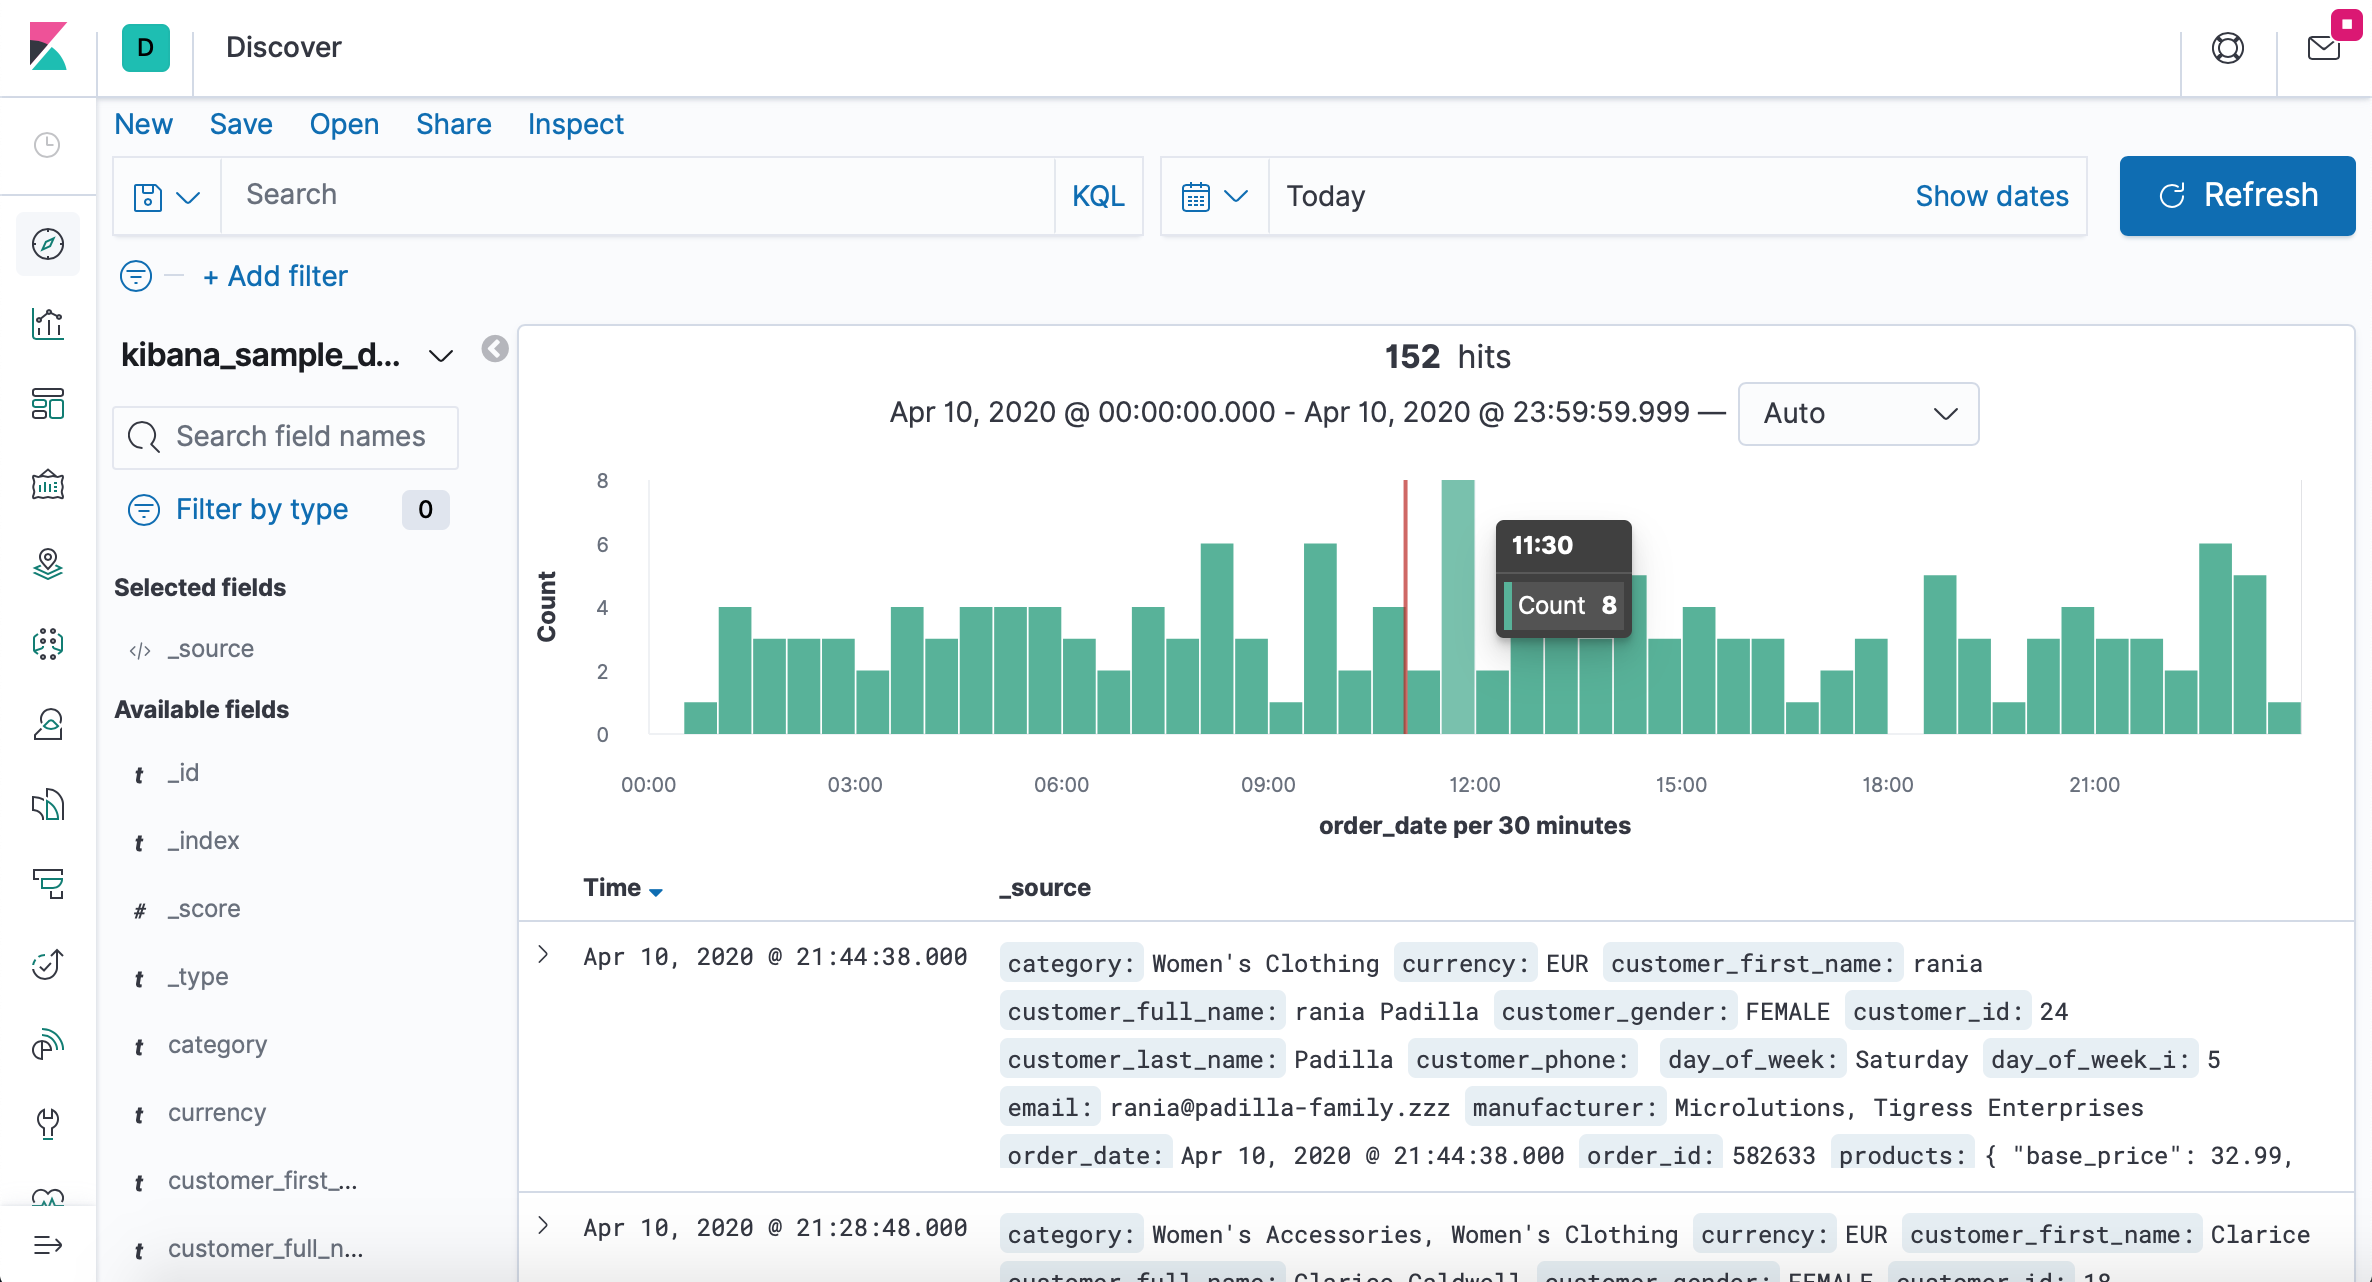
\includegraphics[width=12cm, keepaspectratio]{img/development/Discover-kibana.png}
  \caption{Pestaña Discover del cliente de Kibana}
  \label{fig:kibanadiscover}
\end{figure}

Una vez que ya hemos comprendido, viéndolo en la pestaña de “Discover”, con que clase de datos trabajamos; pasaremos a ver cómo se crean las visualizaciones. Para ello, iremos a la pestaña “Visualization” y lo primero con lo que nos encontramos es con que, al habernos descargado datos de prueba, ya vienen unas predeterminadas. Antes de ponernos a probar a crear una, lo mejor será coger una de estas predeterminada para entender su funcionamiento.

Esta visualización nos muestra una gráfica tipo Pie que viene configurada para que nos muestre el número de ventas en base al género del cliente, ya sea hombre (MALE) o mujer (FEMALE). A mano izquierda vemos que existe también un editor que nos permite configurar la gráfica. Existen dos pestañas dentro de la misma:

\begin{itemize}
    \item \underline{Data:} donde configuraremos qué datos queremos que nos muestre, separados entre metrics y buckets (que explicamos más adelante).
    \item \underline{Options:} como su propio nombre indica, configuraciones opcionales. Por ejemplo, en este caso te permite indicarle donde se desea colocar la leyenda, o si queremos que la gráfica sea rellena o no.
\end{itemize}

\begin{figure}[H]
  \centering
  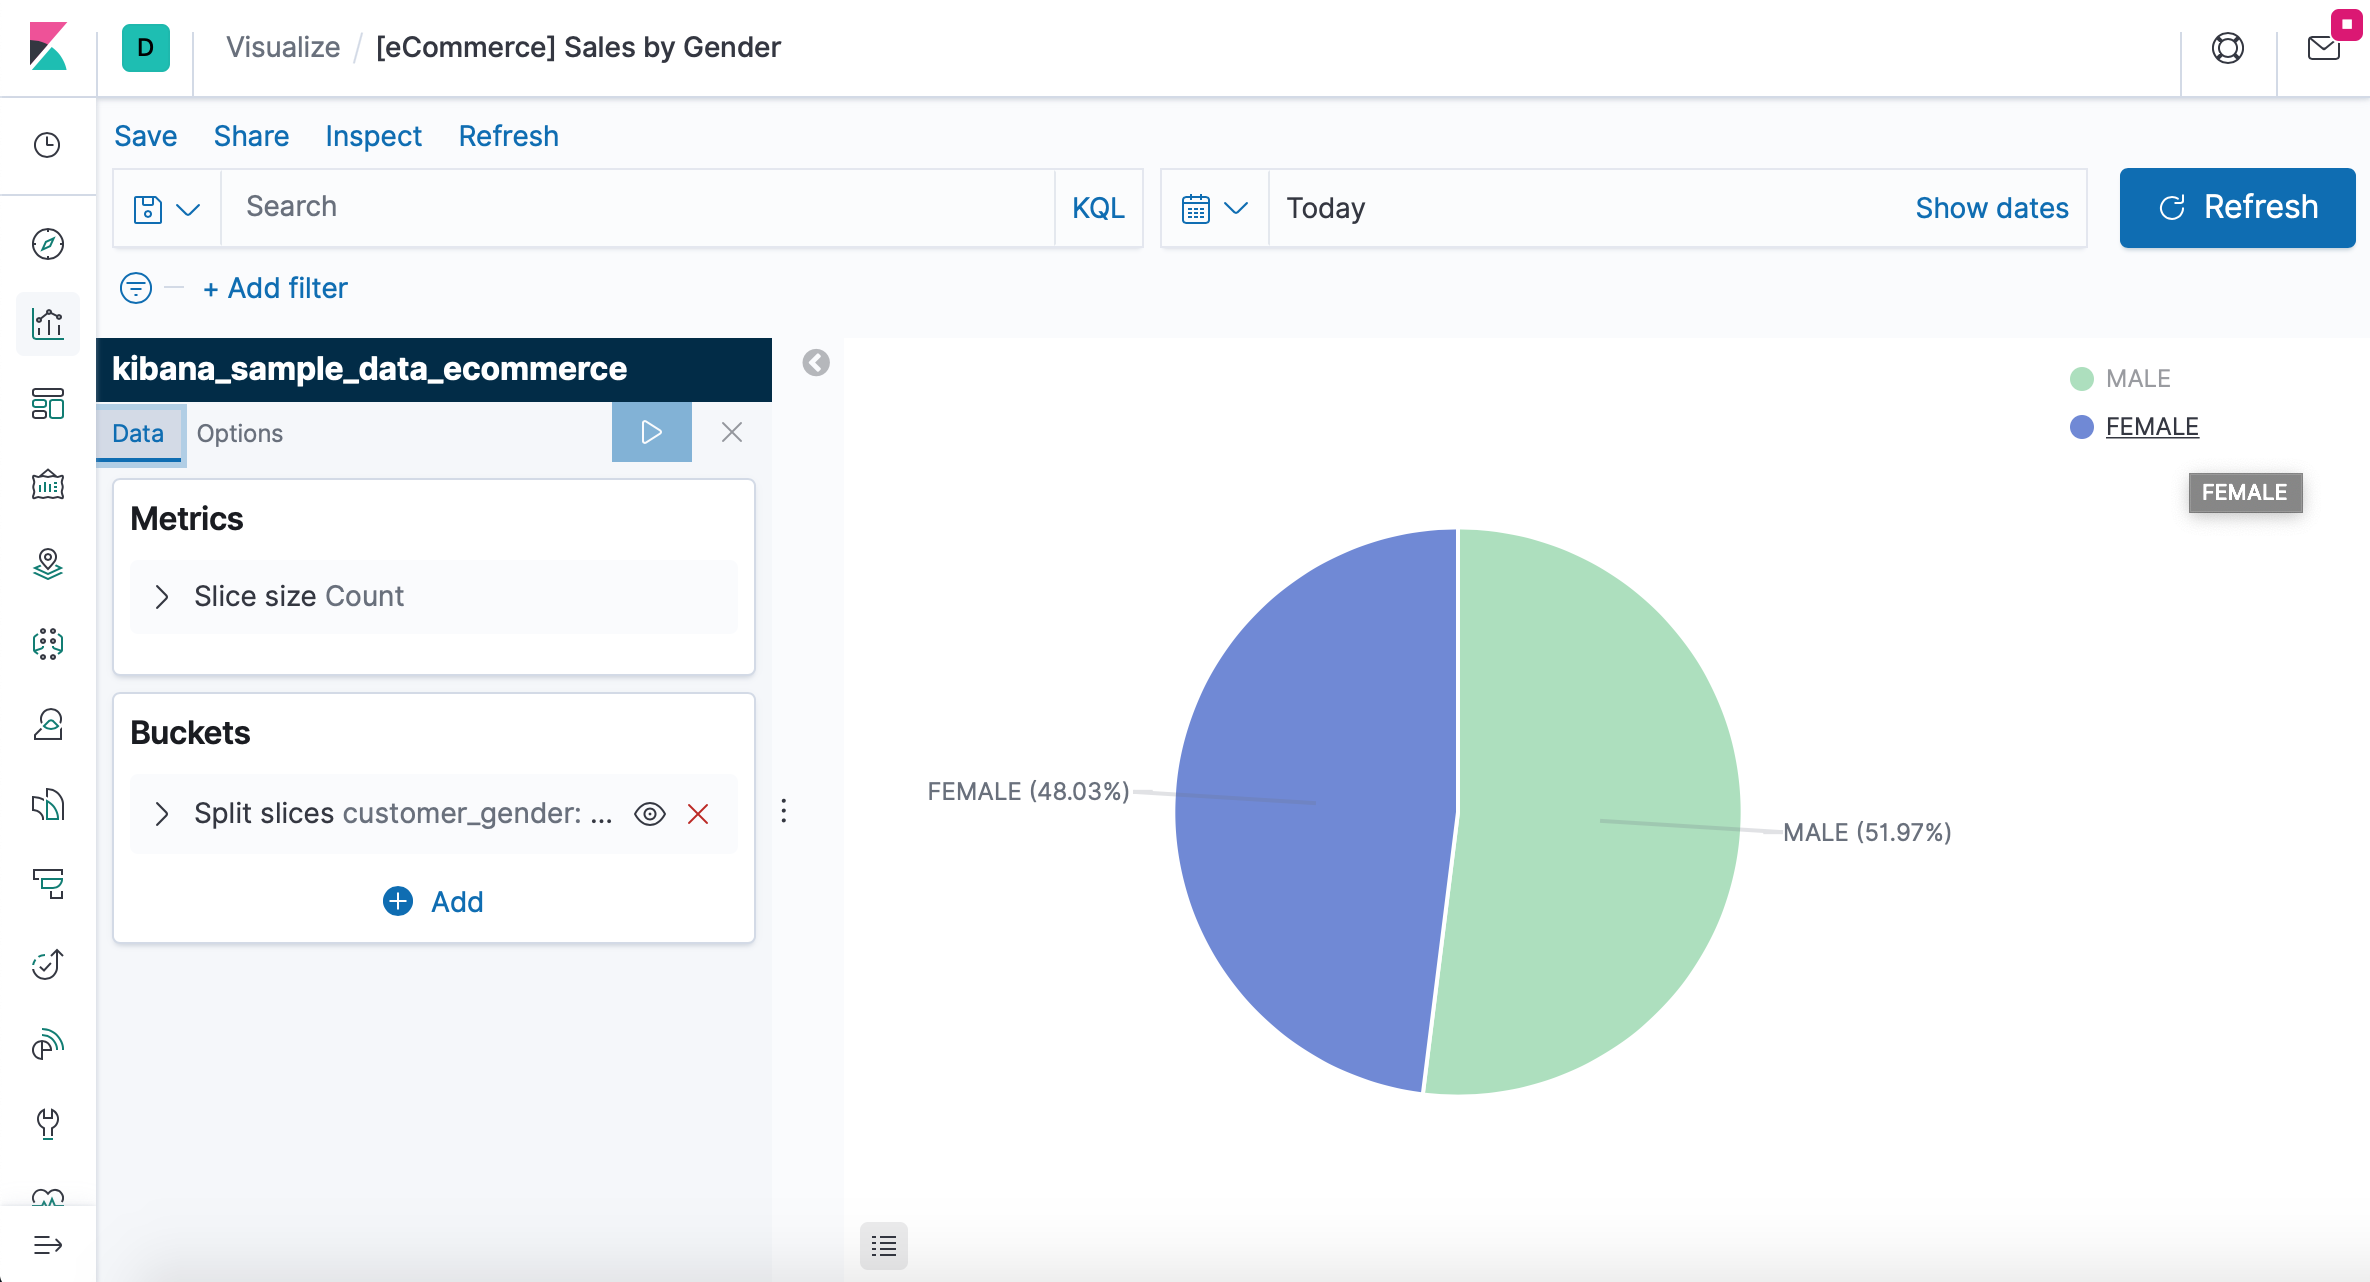
\includegraphics[width=12cm, keepaspectratio]{img/development/Kibana-visualization-pie.png}
  \caption{Visualizacion Pie en el cliente de Kibana}
  \label{fig:kibanapie}
\end{figure}

Ahora que ya entendemos un poco el funcionamiento de las visualizaciones, pasaremos a crear una propia; pero que sea diferente de la anterior. Por ejemplo, nos interesa ver desde qué países se han realizado las ventas. Elegimos “Create Visualization” y seleccionamos, para este caso, la visualización tipo Table. 

Como no nos queremos complicar mucho, lo único que haremos será pedirle que nos muestre la cantidad de ventas que se han realizado en base a los países. Para ello, vamos en la pestaña “Data” y en metrics le indicamos “Count” que nos mostrará la cantidad de ventas. Y luego “Buckets” que nos los clasifique por país. Para ello, se ha de seleccionar en “Aggregations” la opción de “Terms” y luego en “Field” le indicamos que queremos que sea por nombre de país “geoip.region\_name”. Además, nos permite que lo podamos ordenar de mayor a menor o viceversa; o que solo nos muestre, por ejemplo, los 5 primeros. O incluso, darle una etiqueta a los datos que estamos mostrando.

\begin{figure}[H]
  \centering
  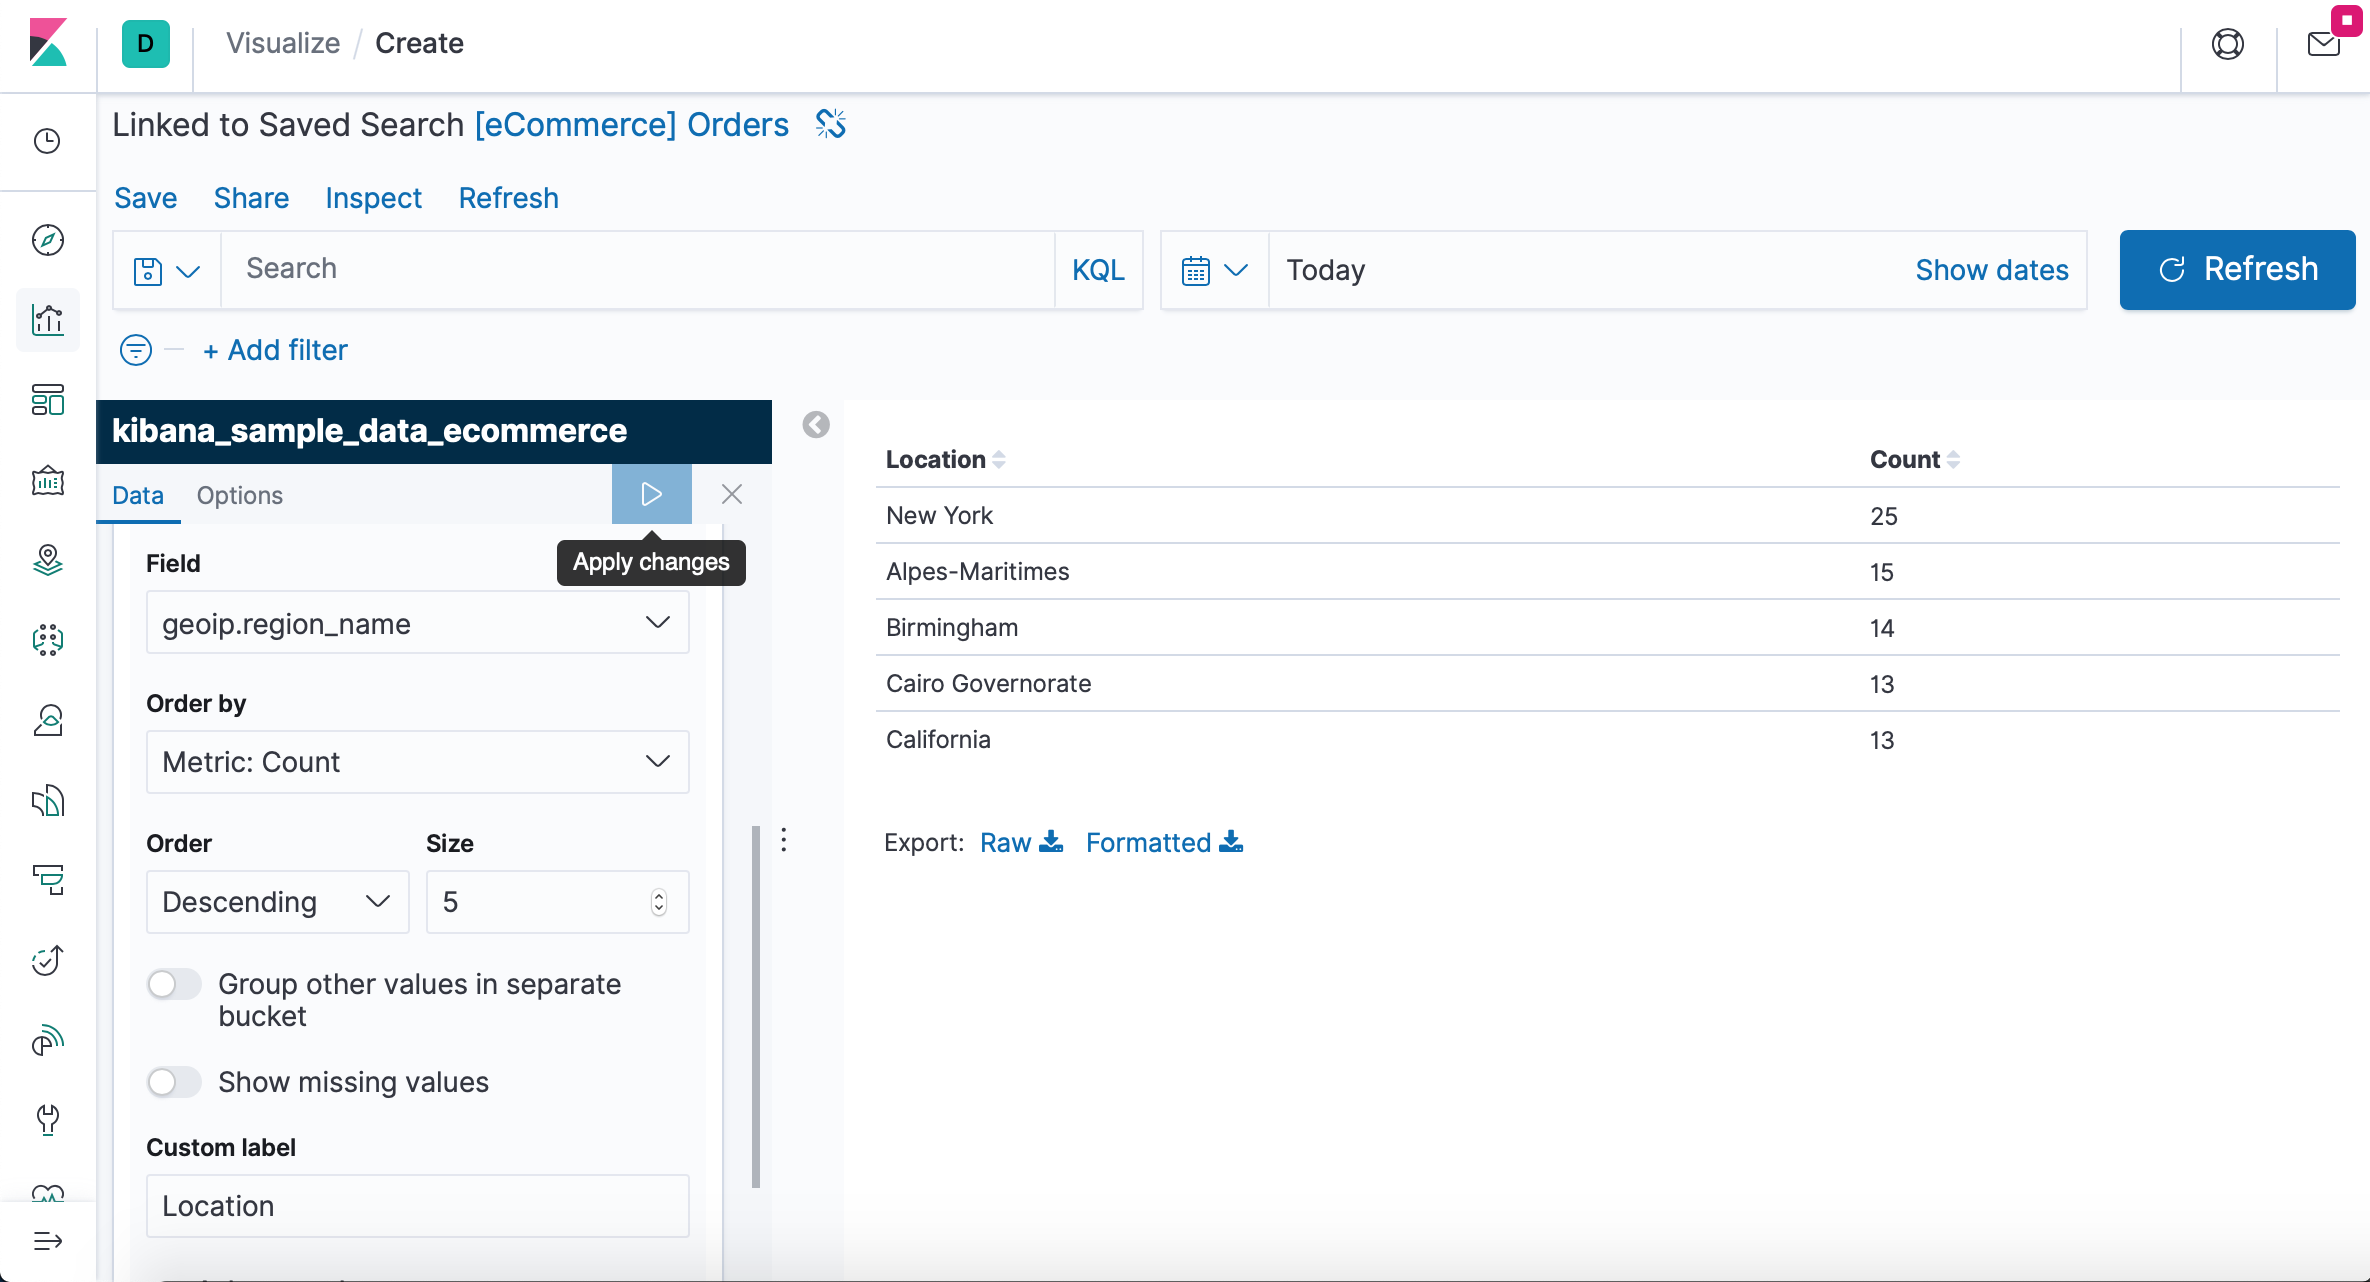
\includegraphics[width=12cm, keepaspectratio]{img/development/kibana-table-editor.png}
  \caption{Creación de Vizualización Table en el cliente de Kibana}
  \label{fig:kibanatable}
\end{figure}

Una vez seleccionado cómo queremos nuestra visualización, solo tenemos que darle a “Apply changes” y se actualizará al instante. Y una vez que tengamos la visualización que queremos, simplemente la guardamos dándole a “Save”.

Después de haber probado alguna visualización y haber creado una propia, nos interesa conocer otra sección interesante y es la que encontramos en la pestaña “Dashboard”. En esta, nos encontramos con que ya existe una predeterminada así que, aunque podemos crear una nueva, la editaremos.

Para entenderlo bien, la dashboard nos muestra en una misma página todas las visualizaciones que tenemos creadas y que queremos que sean mostradas. Lo que nos permite en edición es añadir o eliminar visualizaciones, colocarlas en un sitio u otro; o incluso darles el tamaño que nos interese.

\begin{figure}[H]
  \centering
  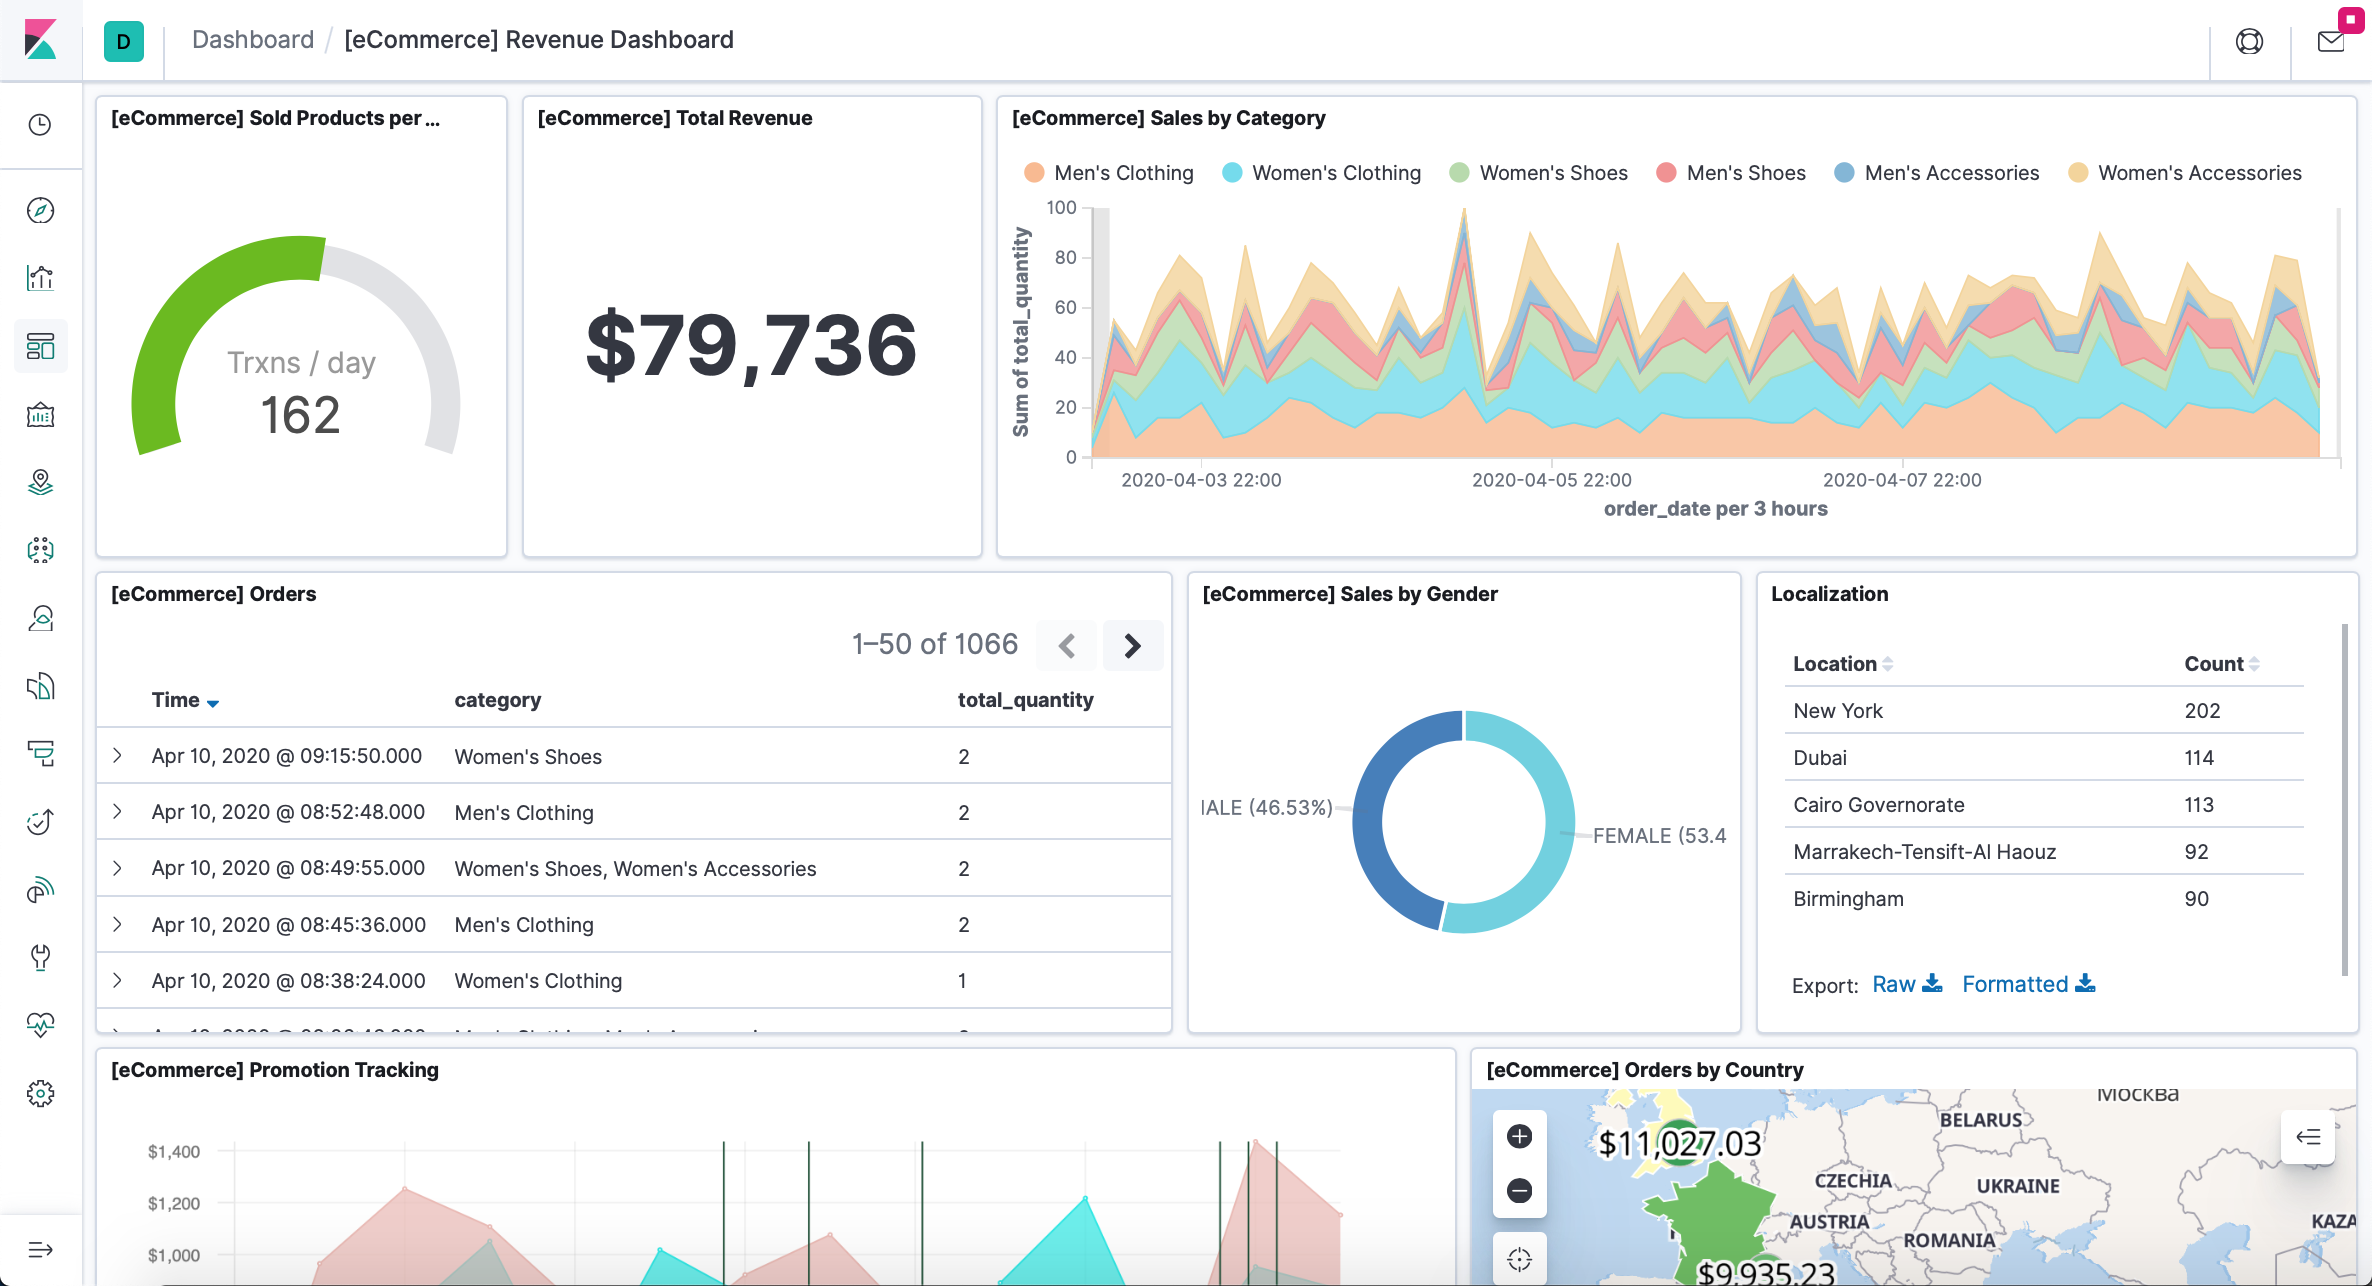
\includegraphics[width=12cm, keepaspectratio]{img/development/kibana-dashboard.png}
  \caption{Dashboard en el cliente de Kibana}
  \label{fig:kibanadashboard}
\end{figure}


%CREANDO ENTORNO DE DESARROLLO
\subsection{Creando el Entorno de Desarrollo}

Ahora que ya entendemos un poco el funcionamiento del cliente de Kibana, pasaremos a crearnos el entorno de desarrollo que utilizaremos para crear nuestro plugin. Este nos permitirá ver en tiempo real los cambios que realicemos.

Siguiendo las indicaciones que podemos encontrar en la sección correspondiente para contribuir en el proyecto (“CONTRIBUTING.md”), dentro del repositorio de kibana.

Una vez tengamos creado nuestro entorno de desarrollo, pasaremos a documentarnos cómo se crean plugin para Kibana. Para ello, elastic no proporciona artículos en su blog de como crear unos plugins básicos. Aunque está un poco obsoleta la documentación, únicamente nos quedaremos con la parte de cómo es la estructura de ficheros.

Por el momento no vamos a detallar el contenido de los ficheros (lo explicaremos más adelante), simplemente nos enfocaremos en qué función tiene cada uno.

Lo primero que haremos será crear un directorio con en nombre de nuestro plugin en “KIBANA\_HOME/plugins”. Dentro de esta habrá dos ficheros:

\begin{itemize}
    \item \underline{package.json:} un simple fichero para nmp donde le indicamos el nombre de nuestro plugin, version, autor, etc. Y sobretodo, las dependencias que necesitamos que nos instale para poder utilizarlas en nuestro proyecto.
    \item \underline{index.js:} este es el módulo principal. En él registramos nuestro plugin indicando el tipo de plugin (dentro de kibana) que es, visualización en este caso; y hacemos referencia al fichero principal.
\end{itemize}

A esto le sigue crear un nuevo directorio con el nombre “public/” que contendrá todos los ficheros de nuestro plugin (controllers, configurations, templates, etc). Antes hemos dicho que desde “index.js” hacíamos referencia a el fichero principal de nuestro plugin, pues es aquí donde lo crearemos.

\begin{itemize}
    \item \underline{public/plugin-name.js:} para el caso de las visualizaciones es donde registramos las diferentes visualizaciones, puede ser una o varias, que vamos a añadir en kibana a través de nuestro plugin.
\end{itemize}

Todos los ficheros anteriormente mencionados son los principales para el funcionamiento de esto; pero a mayores se le pueden añadir más ficheros. Algunos ejemplos opcionales:

\begin{itemize}
    \item \underline{public/plugin-name-controller.js:} como su propio nombre indica, sería el controlador de nuestro plugin. En el contiene toda la parte lógica de nuestra visualización.
    \item \underline{public/plugin-name.html:} template del plugin.
    \item \underline{public/plugin-name.less:} hoja de estilo del plugin.
    \item \underline{public/options-template.html:} template para la pestaña “options” del editor.
\end{itemize}

De forma más visual, podemos decir que la estructura de ficheros para crear un plugin para kibana es la siguiente:


\begin{lstlisting}[frame=single]
KIBANA_HOME/plugins
|___plugin-name
    |___package.json
    |___index.js
    |___public
        |___plugin-name.js
        |___plugin-name-controller.js
        |___plugin-name.html
        |___plugin-name.less
        |___options-template.html

\end{lstlisting}



%TESTEANDO BIBLIOTECA PARA LAS VISUALIZACIONES
\subsection{Testeando Biblioteca para las Visualizacione}

Al igual que necesitamos conocer el funcionamiento de kibana, también necesitamos tener unos conceptos básicos sobre los componente visuales que vamos a incorporar para nuestras visualizaciones para kibana.

La opcion de usar Babiaxr ha sido muy acertada, ya que permite crear gráficas, a partir de datos proporcionados, dentro de un escenario webVR. Así que antes de nada, analizaremos lo que nos ofrece y cómo se crean.

Dentro del repositorio de babiaxr podemos ver los distintos tipos de componentes que tienen creados. Dichas componentes han sido creadas a partir del framework a-frame (ver ...).

Lo primero que haremos será probar los diferentes componentes que tienen: “geopiechart”, “geosimplebarchar”, “geo3dbarchart” y “geobubblechart”. Todas ellas se pueden probar desde su web.

\begin{figure}[H]
  \centering
  \minipage{0.32\textwidth}
  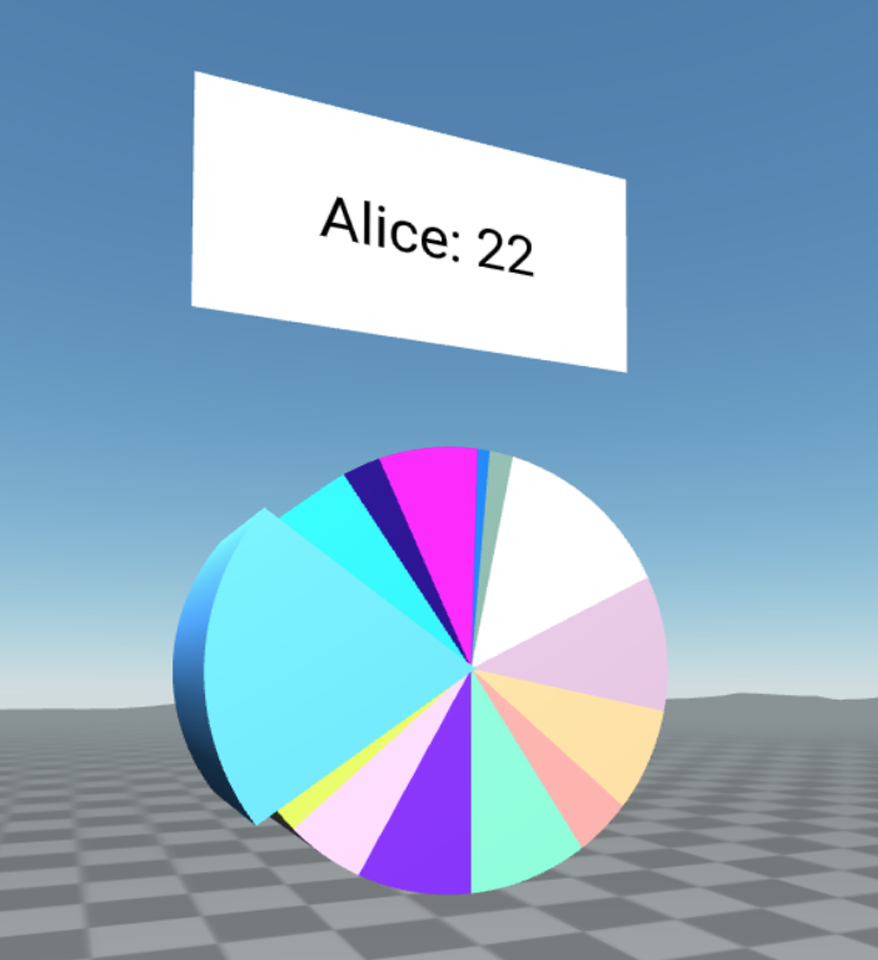
\includegraphics[width=5cm, keepaspectratio]{img/development/babiaxr-pie.png}
  \caption{Geopiechart}
  \label{fig:babiaxrgeopiechart}
  \endminipage\hfill
  \minipage{0.32\textwidth}
  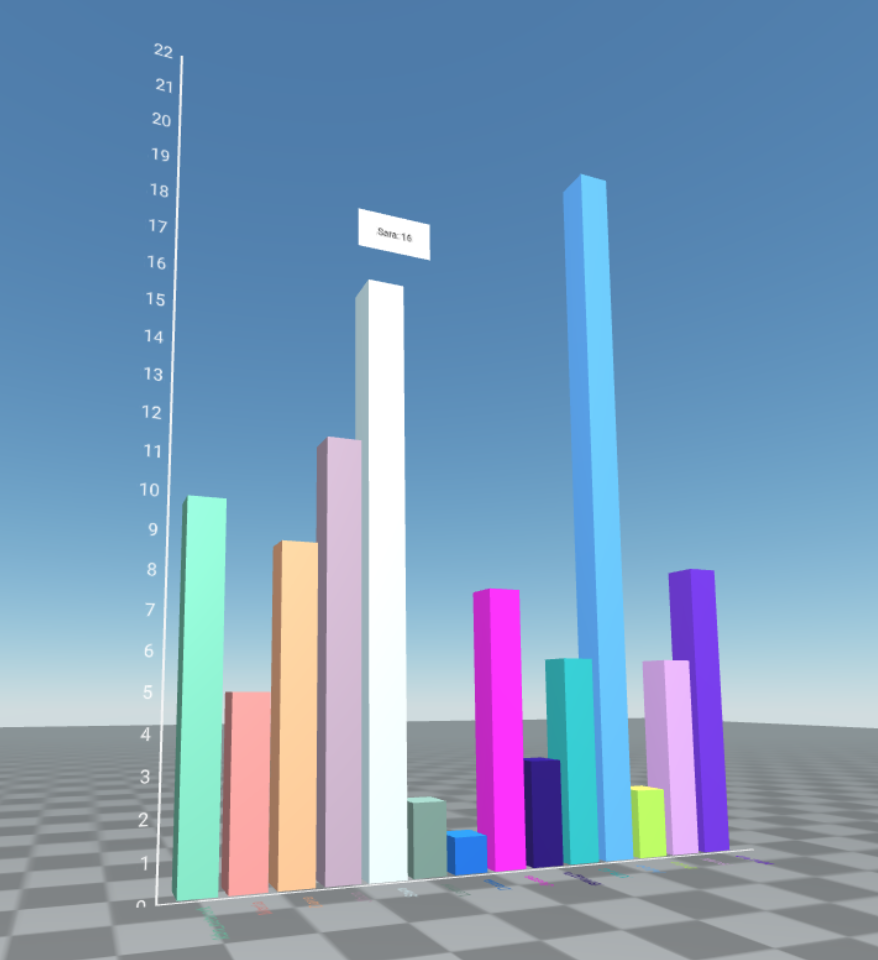
\includegraphics[width=5cm, keepaspectratio]{img/development/babiaxr-simplebar.png}
  \caption{Geosimplebarchart}
  \label{fig:babiaxrgeosimplebarchart}
  \endminipage\hfill
  \minipage{0.32\textwidth}
  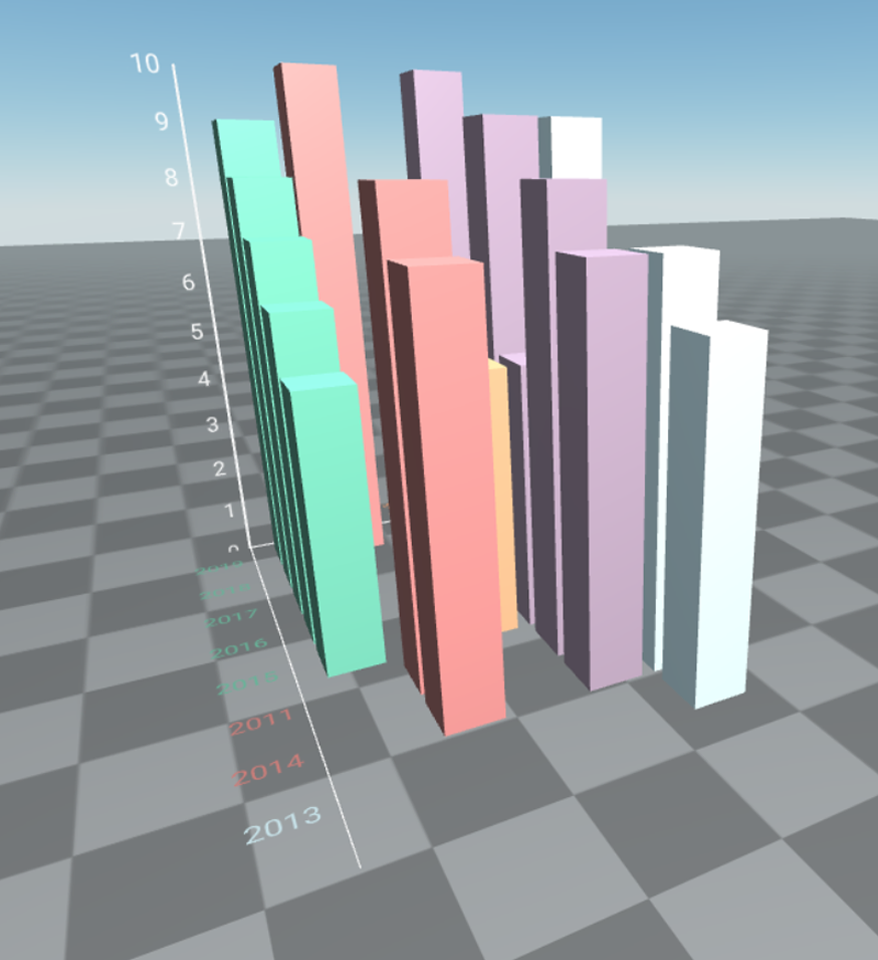
\includegraphics[width=5cm, keepaspectratio]{img/development/babiaxr-3dbar.png}
  \caption{Geo3dbarchart}
  \label{fig:babiaxrgeo3dbarchart}
  \endminipage\hfill
\end{figure}

\begin{figure}[H]
  \centering
  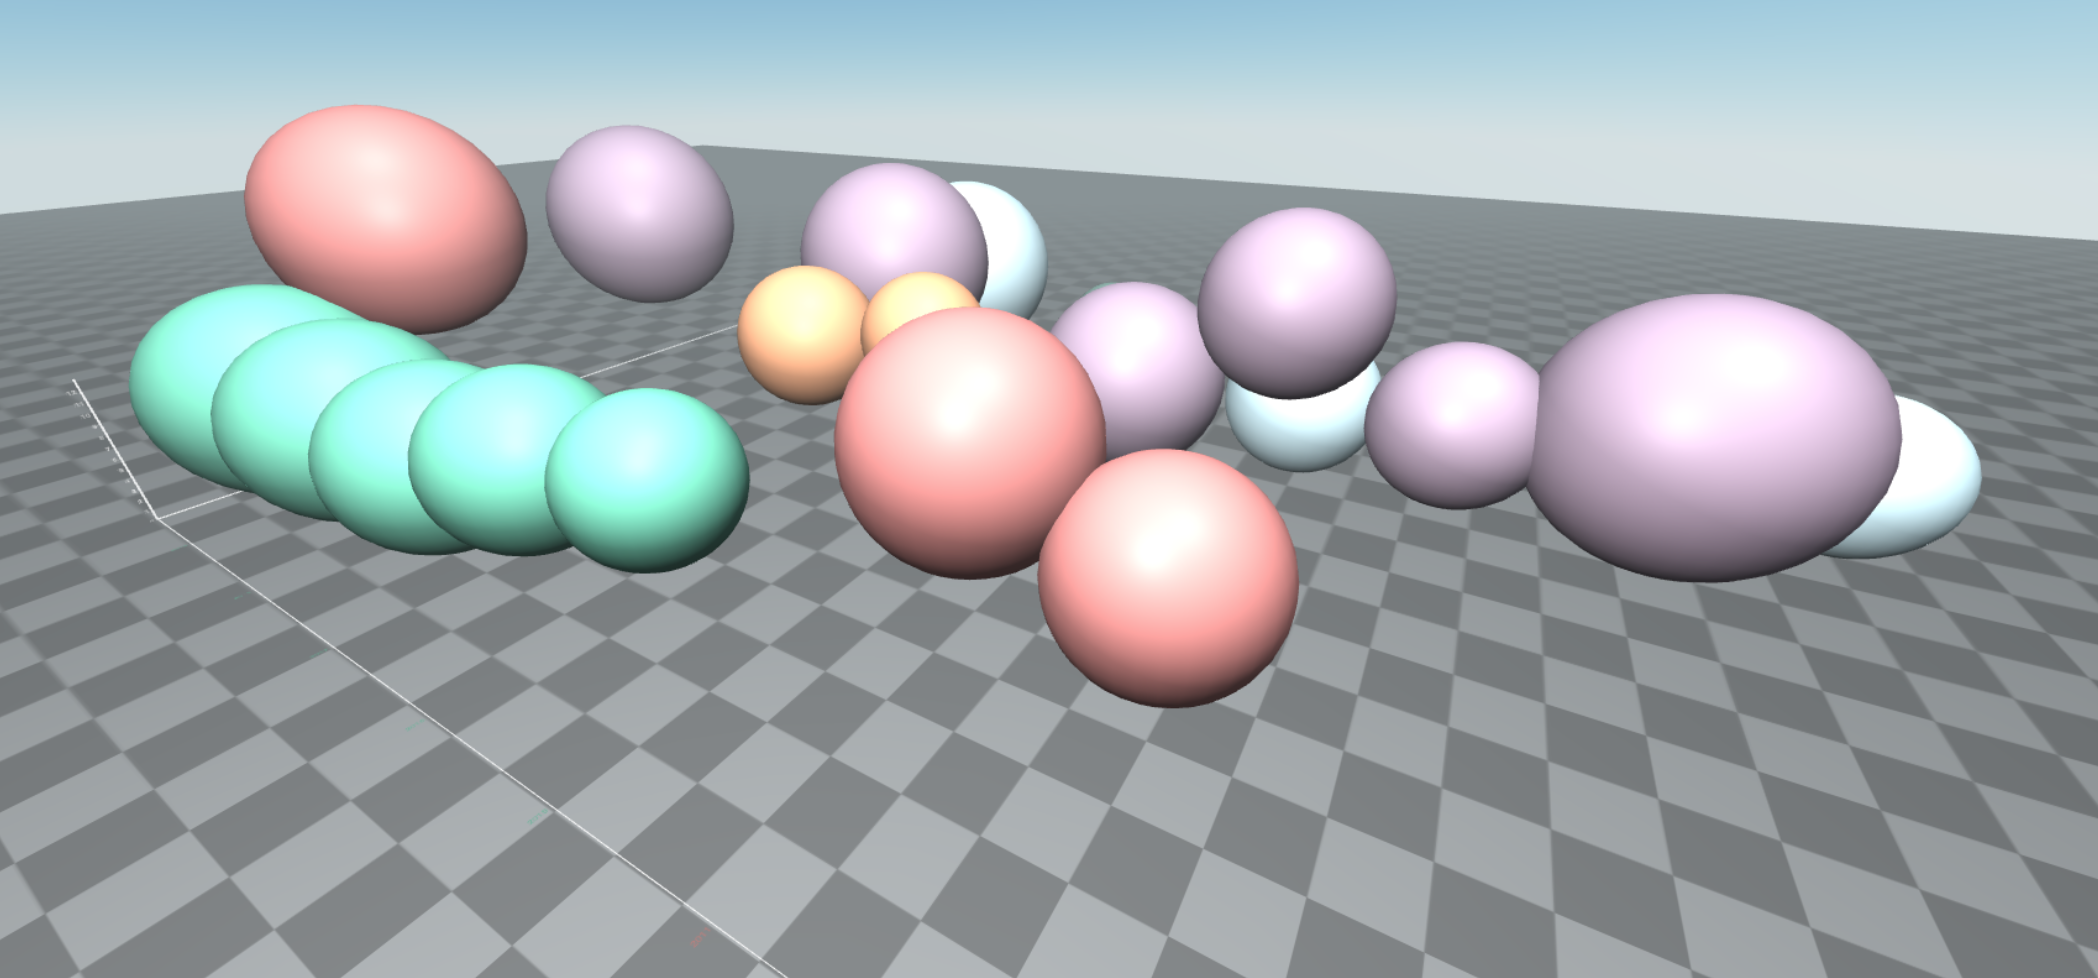
\includegraphics[width=10cm, keepaspectratio]{img/development/babiaxr-bubble.png}
  \caption{Geobubblechart}
  \label{fig:babiaxrgeobubblechart}
\end{figure}


Una vez que hemos visto lo que hace, probaremos a crear nuestro propio escenario con la componente “geopiechart” con datos que le daremos de forma manual. Para ello, nos apoyaremos en la documentación que nos facilita su autor.

\begin{lstlisting}[frame=single]
<a-entity geopiechart='legend: true;
    data: [{"key":"Andrea","size":9},{"key":"URJC","size":8},
    {"key":"ETSIT","size":7},{"key":"kibana","size":6},
    {"key":"elasticsearch","size":5},{"key":"Jesus","size":8},
    {"key":"David","size":7}]'
position="-3 5 15" rotation="90 0 0"></a-entity>

\end{lstlisting}

Obteniendo como resultado:

\begin{figure}[H]
  \centering
  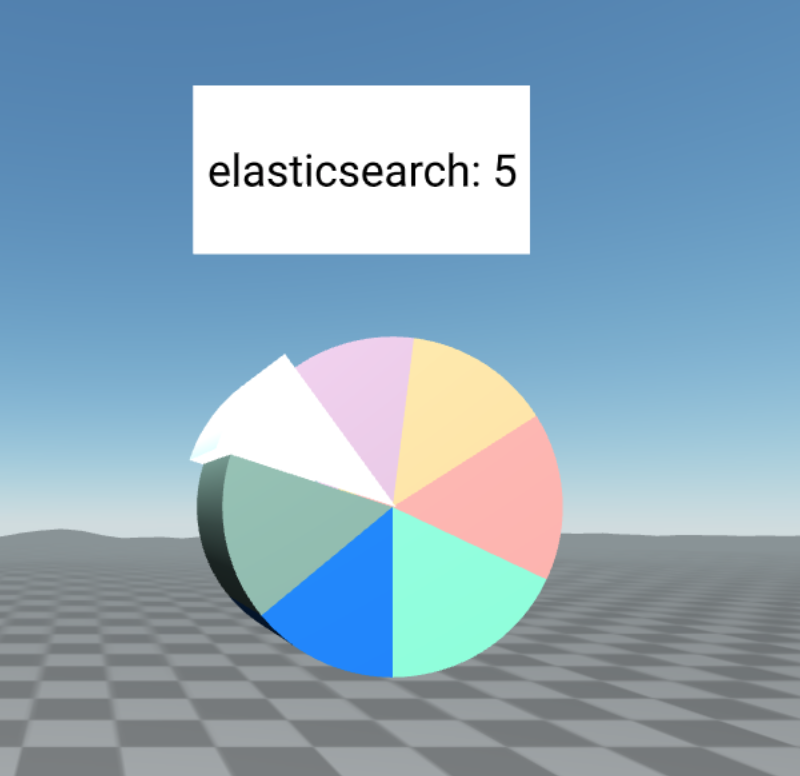
\includegraphics[width=6cm, keepaspectratio]{img/development/prueba-babiaxr.png}
  \caption{Pie Chart de Prueba}
  \label{fig:pruebababiaxr}
\end{figure}

Con todo esto, ya podemos proceder a crear nuestro primer plugin.


%%%%%%%%%%%
% SPRINT 1
%%%%%%%%%%%

\section{Sprint 1: Primeros Plugins de Visualización }
\label{sec:sprint1}

%%%%%%%%%%%
% SPRINT 2
%%%%%%%%%%%

\section{Sprint 2: Visualización con datos Elasticseach }
\label{sec:sprint2}
\subsection{Editor y Schemas}
Hasta este punto hemos aprendido a crear un plugin simple para kibana e integrarlo con aframe. El siguiente paso será aprender a sacar datos de elasticsearch y poder dibujar un figura de aframe, en este caso un cubo, con las dimensiones que le obtenemos de dichos datos. Para ello, seguiremos los siguiente pasos:
\begin{enumerate}
    \item Añadir Editor y Schemas.
    \item Construir Visualización que muestre datos.
    \item Integración de Aframe con datos.
\end{enumerate}

Antes de ponernos a crear una nueva visualización donde nos muestre datos de elasticsearch, necesitamos un editor que nos permita seleccionar los datos que queremos mostrar. 

Comenzaremos creando el diseño de nuestro editor. Kibana nos permite seleccionar dos tipo de datos: metrics y buckets.
\begin{itemize}
    \item \underline{metrics:}hace referencia a datos que se pueden calcular, por ejemplo, media, máximo, sumatorio, etc.
    \item \underline{buckets:}refiere a un conjunto de datos que no se pueden calcular, por ejemplo, fechas, sucursales, tipos, etc.
\end{itemize}

Como el objetivo final de este sprint es crear una visualización que nos muestre un cubo, determinamos que necesitaremos 3 datos metrics que serán los datos que usaremos para crear las dimensiones del cubo que dibujaremos más adelante.

Estos datos vienen estructurados dentro de Schemas que el propio Kibana permite declarar a la hora de crear la visualización para luego registrarla. Para ello, añadiremos las siguiente líneas en “kbn\_aframe.js”:

Antes de nada, importamos los correspondientes paquetes que nos permite declarar los schemas e indicar el tipo de dato que vamos a usar, en este caso metrics.

\begin{lstlisting}[frame=single]
import { Schemas } from 'ui/vis/editors/default/schemas';
import { AggGroupNames } from 'ui/vis/editors/default';
\end{lstlisting}

Una vez importado, añadiremos nuevos parámetros dentro de la función createBaseVisualization():

\begin{lstlisting}[frame=single]
schemas: new Schemas([
        {
          group: AggGroupNames.Metrics,
          name: 'x-axis',
          title: 'X-axis',
          min: 1,
          max: 1,
          aggFilter: ['count', 'avg', 'sum', 'min', 'max', 
          'cardinality', 'std_dev']
        },
        {
          group: AggGroupNames.Metrics,
          name: 'y-axis',
          title: 'Y-axis',
          min: 1,
          max: 1,
          aggFilter: ['count', 'avg', 'sum', 'min', 'max', 
          'cardinality', 'std_dev']
        },
        {
          group: AggGroupNames.Metrics,
          name: 'z-axis',
          title: 'Z-axis',
          min: 1,
          max: 1,
          aggFilter: ['count', 'avg', 'sum', 'min', 'max', 
          'cardinality', 'std_dev']
        }
      ]),
\end{lstlisting}

Parámetros utilizados:
\begin{itemize}
    \item \underline{group:} indica el tipo de dato: metric o bucket.
    \item \underline{name:} nombre que recibirá el dato.
    \item \underline{title:} el título que mostrará en el editor.
    \item \underline{min:} indica el mínimo de datos que tenemos usar.
    \item \underline{max:} indica el máximo de datos que podemos usar.
    \item \underline{aggFilter:} aquí podemos indicarle qué tipos de dato, en este caso tipos de métricas, queremos usar.
\end{itemize}

Al instante de añadir esto, obtenemos como resultado un editor como el que vemos a continuación:

\begin{figure}[H]
  \centering
  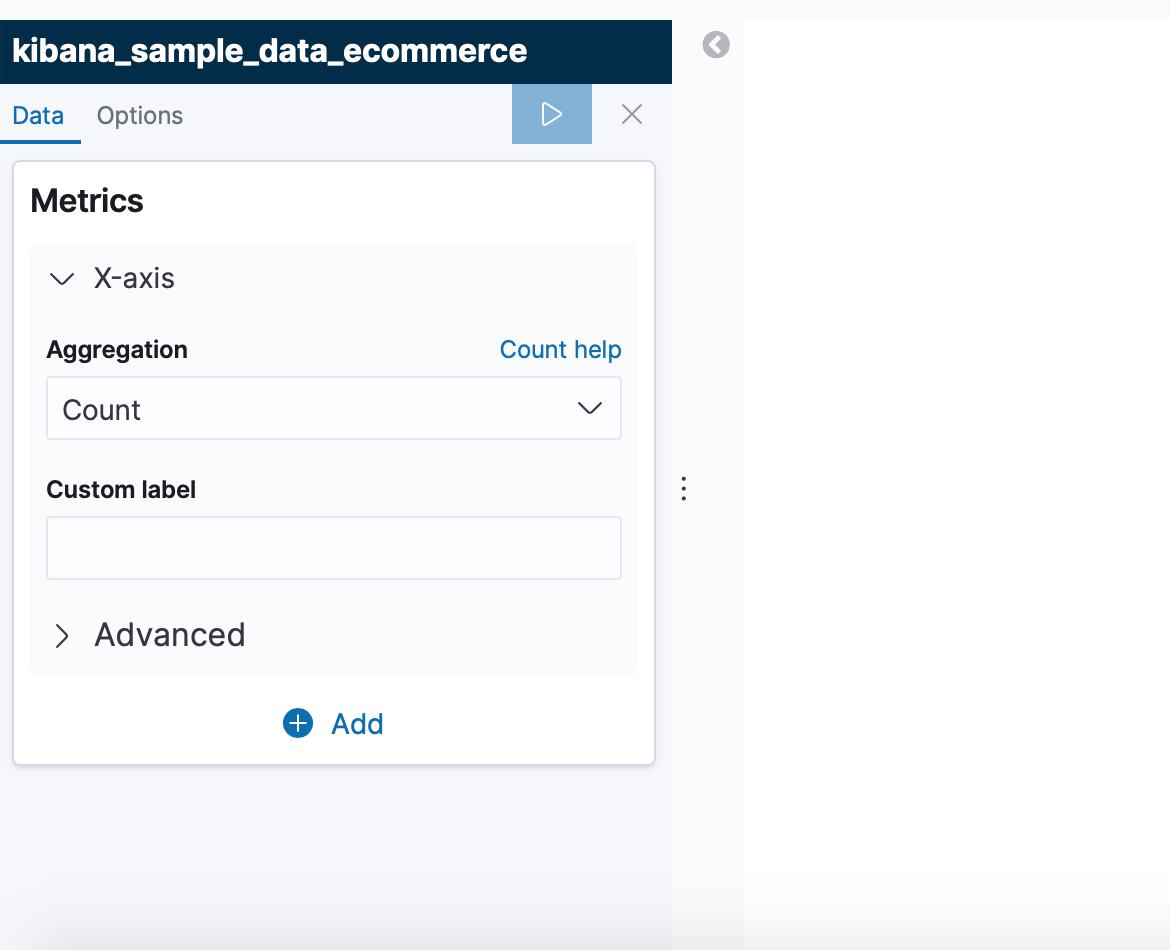
\includegraphics[width=10cm, keepaspectratio]{img/development/editor-resultado.png}
  \caption{Resultado del Editor}
  \label{fig:editor}
\end{figure}

\subsection{Plugin Simple con datos}
Ahora que ya podemos elegir los datos en el editor de Kibana, el siguiente paso es conseguir que la visualización muestre dichos datos de forma sencilla.

Para esto debemos haber aprendido, como se vió en el sprint anterior, el funcionamiento de creación y renderizado para entender dónde Kibana recibe los datos de elasticsearch. Así que lo primero que tenemos que hacer es encontrar dónde recibimos los datos que pedimos con el editor.

Si revisamos el esquema del proceso de creación de una visualización (ver capitulo), podemos suponer que los datos que recibimos vendrán en la variable visData. Lo comprobaremos de la siguiente forma:

\begin{lstlisting}[frame=single]
  render(visData, status) {
      if (visData) {
        console.log(visData);
      }
\end{lstlisting}

Con esto podremos ver que datos recibimos en la consola del navegador.

\begin{figure}[H]
  \centering
  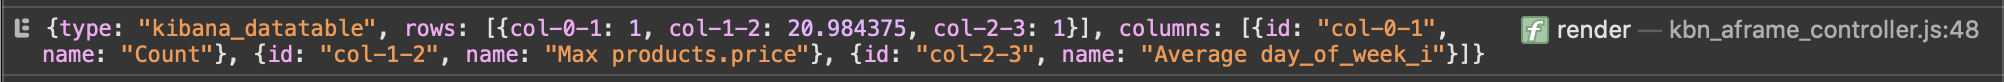
\includegraphics[width=16cm, keepaspectratio]{img/development/captura-visData.png}
  \caption{Captura de visData en la consola}
  \label{fig:visData}
\end{figure}
Esto nos sirve para analizar en cómo es el formato de los datos recibidos de elasticsearch, para luego extraer los datos que nos interesa mostrar. 

En primer lugar, vemos que se divide en 3 registros: 
\begin{itemize}
    \item \underline{type:} tipo del archivo. En este caso, kibana\_datatable.
    \item \underline{rows:} contiene únicamente los datos obtenidos en formato registro en la que la clave con la forma col-X-X que indica la posición; y el valor con el dato obtenido.
    \item \underline{columns:} contiene las etiquetas que hacen referencia a los datos obtenidos. Vienen en forma de array de registros, donde el id indica la posición del dato; y el name indica el nombre del valor. 
\end{itemize}
Analizando todo esto sacaremos los datos, con sus nombres, para guardarlo en la variable metrics.

\begin{lstlisting}[frame=single]
     const table = visData;
     const metrics = [];

      //get metrics
      table.columns.forEach((column, i) => {
        var value;
        const name = column.name;
        const id = column.id;
        table.rows.forEach(row => {
          if (row[id]){
            value = Math.round(row[id]*100)/100;
          }
        });

       metrics.push({
          name: name,
          value: value
        });
      });
\end{lstlisting}
Tras esto, lo añadimos a la visualización, de forma simple, de la siguiente forma:
\begin{lstlisting}[frame=single]
      //render metric in vis
      metrics.forEach((metric, i) => {
        const metricDiv = document.createElement('div');
        metricDiv.className = 'myvis-metric-div';
        metricDiv.innerHTML = `<b>${metric.name}:</b> 
        ${metric.value}`;
        metricDiv.setAttribute('style', `font-size: 
        ${this.vis.params.fontSize}pt`);
        this.container.appendChild(metricDiv);
      });
\end{lstlisting}
Como resultado obtenemos las figuras, que agregamos anteriormente en el capítulo anterior, seguido de los 3 valores que pedimos desde el editor.
\begin{figure}[H]
  \centering
  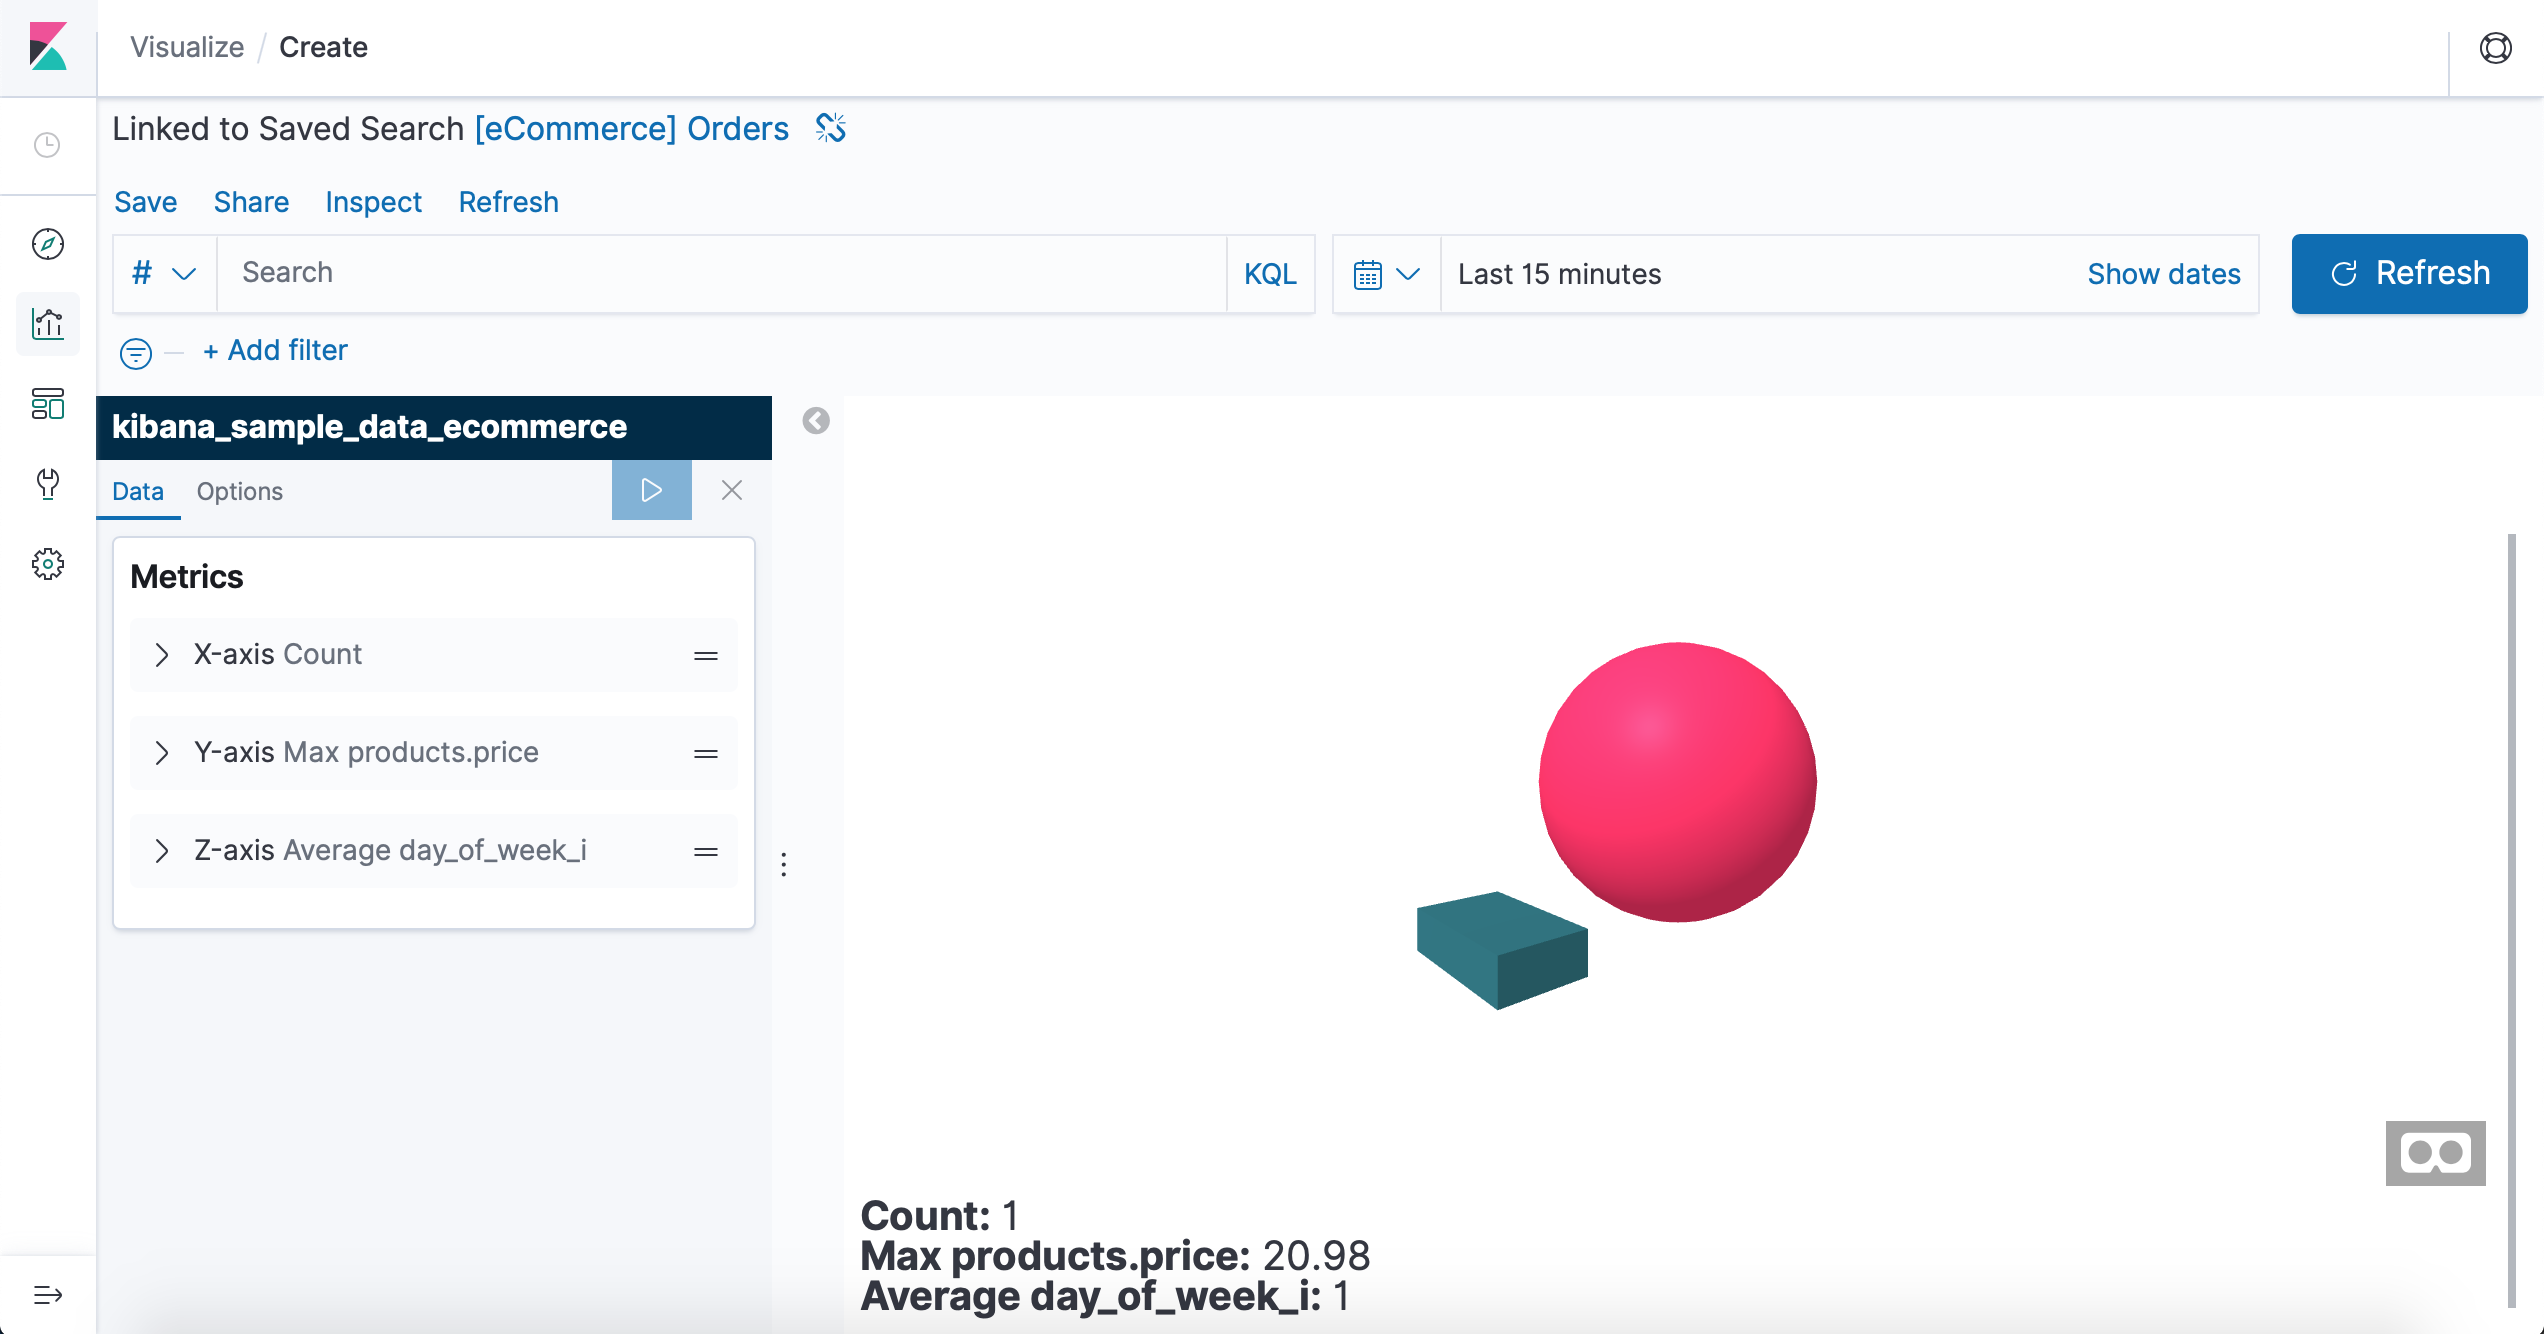
\includegraphics[width=16cm, keepaspectratio]{img/development/resultado-simple-data.png}
  \caption{Resultado Visualización con datos}
  \label{fig:simplewithdata}
\end{figure}


\subsection{Integración de A-frame con datos}
Ahora que ya hemos aprendido a obtener los datos que pedimos a elasticsearch para incluirlos en nuestra visualización, el siguiente paso es saber añadir estos datos para poder crear las figuras en base a estos datos.

Únicamente nos centraremos en crear el cubo tomando como valores las 3 métricas que pedimos desde el editor. Para ello, tenemos dos opciones:
\begin{enumerate}
    \item Insertar los datos al html usando angularJS.
    \item Crear la figura directamente desde el controller usando a-frame con javascript.
\end{enumerate}
Analizando un poco como kibana crea sus visualizaciones predeterminadas, creo que la mejor opción es la segunda y así nos ahorramos tener que usar más bibliotecas.

Por eso, eliminaremos el archivo “index.html”, eliminamos la línea donde importamos dicho archivo y cambiamos la siguiente línea de render():

\begin{lstlisting}[frame=single]
    this.container.innerHTML = '';
\end{lstlisting}

Ahora crearemos el escenario justo de donde añadimos las métricas obtenidas de elasticsearch.

\begin{lstlisting}[frame=single]
     //Creando escenario
      var escena = document.createElement('a-scene');
      escena.setAttribute('embedded', true);
\end{lstlisting}

El siguiente paso será añadir las figuras. Empezaremos por dibujar una esfera usando las primitivas que tiene a-frame. Usaremos los mismos valores que teníamos en “index.html” pero variando algún dato al gusto. Por el momento solo le añadimos los datos de forma manual porque lo único que queremos es probar cómo podemos crear una figura de esta forma.

Lo creamos de la siguiente forma:

\begin{lstlisting}[frame=single]
     // entity primitive
      var entidad = document.createElement('a-entity');
      entidad.setAttribute('geometry', {
        primitive: 'sphere',
        radius: 1.25
      });
      entidad.setAttribute('position', {
        x: -2.5,
        y: 1,
        z: -5
      });
      entidad.setAttribute('material',{
        color: '#EF2D5E'
      });
      entidad.setAttribute('shadow', true);

      escena.appendChild(entidad);
\end{lstlisting}

Esta última línea, añade la figura en el escenario anteriormente creado.

Ahora que está creado todo la escena con la figura, la añadimos el contenedor de la visualización para que nos la muestre en Kibana.

\begin{lstlisting}[frame=single]
     this.container.appendChild(escena);
\end{lstlisting}

Obteniendo como resultado la siguiente visualización.

%\begin{figure}[H]
  %\centering
  %\includegraphics[width=16cm, keepaspectratio]{img/development/}
  %\caption{Esfera A-Frame con Javascript}
 % \label{fig:onlysphere}
%\end{figure}

Una vez hemos conseguido que nos dibuje la esfera, haremos el mismo procedimiento para crear el cubo pero con un par de variaciones:

\begin{enumerate}
    \item Usaremos el cubo que creamos por componente.
    \item Añadiremos los datos obtenidos de elasticsearch.
\end{enumerate}

Como usaremos el componente, revisaremos que “box.js” este importado en el controlador.

Ahora, declaramos un array con las dimensiones que vamos a usar para crear el cubo. 

\begin{lstlisting}[frame=single]
     const axis = [];
\end{lstlisting}
Y añadimos los valores en la variable axis tras añadirlo también en metrics.
\begin{lstlisting}[frame=single]
       // add axis
        axis.push(value);
\end{lstlisting}
Por último, solo nos queda crear la figura de la misma forma y añadirlo en la escena:
\begin{lstlisting}[frame=single]
     // entity con box.js
      var caja = document.createElement('a-entity');
      caja.setAttribute('box', {
        height: axis[0]/10, //0.5
        width: axis[1]/10, //0.25
        depth: axis[2]/10, //1
      });
      caja.setAttribute('position', {
        x: 0,
        y: 1,
        z: -5
      });
      caja.setAttribute('rotation', {
        x: 0,
        y: -45,
        z: 0
      });
      caja.setAttribute('material', 'color', '#4CC3D9');

      escena.appendChild(caja);
\end{lstlisting}
Como se ve, la diferencia con la esfera es que creamos un a-entity con el atributo ‘box’ y no ‘geometry’ y dándole los datos que declaramos en el constructor de box.js.

Con esto, obtenemos como resultado un cubo que varía en base a los datos que le pedimos a elasticsearch.

\begin{figure}[H]
  \centering
  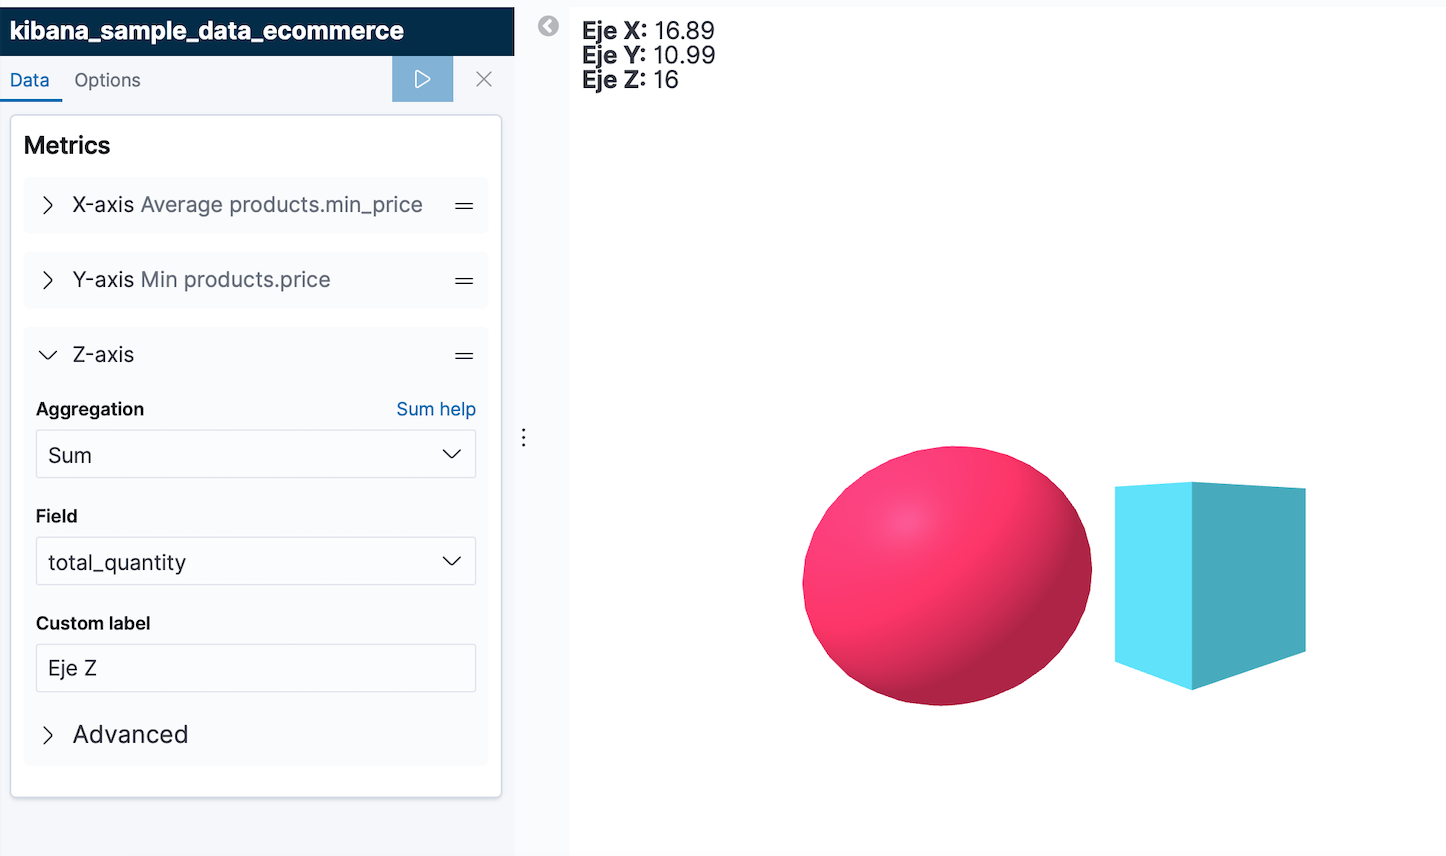
\includegraphics[width=16cm, keepaspectratio]{img/development/box_with_data.png}
  \caption{Resultado de integración de A-Frame con datos}
  \label{fig:boxwithdata}
\end{figure}

%\begin{lstlisting}[frame=single]
%\end{lstlisting}

%\begin{figure}[H]
%  \centering
%  \includegraphics[width=16cm, %keepaspectratio]{img/development/}
%  \caption{}
%  \label{fig:}
%\end{figure}

% Esto va al final de todo.
\end{document}